%%%%%%%%%%%%%%%%%%%%%%%%%%%%%%%%%%%%%%%%%%%%%%%%%%%%%%%%%%%%%%%%%%
%                           Document style
%%%%%%%%%%%%%%%%%%%%%%%%%%%%%%%%%%%%%%%%%%%%%%%%%%%%%%%%%%%%%%%%%%
\documentclass[12pt]{article}

% Importing report style and the first pages 
%%%%%%%%%%%%%%%%%%%%%%%%%%%%%%%%%%%%%%%%%%%%%%%%%%%%%%%%%%%%%%%%%%
%                       Main document style 
%%%%%%%%%%%%%%%%%%%%%%%%%%%%%%%%%%%%%%%%%%%%%%%%%%%%%%%%%%%%%%%%%%

% Importing user packages (librarys for different functions and commands) 
\usepackage[utf8]{inputenc}         % interprets charecters as if they comply to ASCII standards
\usepackage{todonotes}              % to do notes 
\usepackage{subfiles}               % add subfiles
\usepackage[T1]{fontenc}            % text font
\usepackage{lmodern}                % font
\usepackage{pdfpages, pdflscape}    % add pdf's 
\usepackage{gensymb, textcomp}      % add symbols
\usepackage{lastpage}               % get the last page number 
\usepackage{graphicx}               % add images 
\usepackage{tabularx}               % add tables 
\usepackage{mathtools}              % math
\usepackage{listings}               % add lists (code)
\usepackage{enumitem}               % options for enumerate
\usepackage{setspace}               % define size of space (infinite) 
\usepackage{xcolor}                 % colors
\usepackage{fancyhdr}               % to get fancy headers
\usepackage [background=black, arrow=red, text=white]{callouts}      % add callouts 
\usepackage{wrapfig}                % positioning figures
\usepackage{subcaption}             % position mulitple figures 
\usepackage{tikz}
\usepackage{upquote}
\usepackage{tikz}                   % text on top of images
\usepackage{amsmath, amssymb}

\usepackage[document]{ragged2e}
\usepackage{float}
\usepackage{csvsimple,longtable,booktabs}
\usepackage{ titlesec}
\usepackage[autostyle]{csquotes}
% \usepackage[
% backend=biber,
% style=style=authoryear,
% ]{biblatex}
\usepackage{url}


% page settings
\setlength{\marginparwidth}{2cm}    % margins
\usepackage[a4paper,left=2.5cm,right=2.5cm,top=2.5cm,bottom=4cm]{geometry}                 % dimensions 
\setlength\parindent{0pt}
\setlength{\parskip}{1em}
\setcounter{MaxMatrixCols}{20}

\renewcommand{\contentsname}{Contents} % content table 

\setlength{\headheight}{35.372pt} % header height

\cfoot\thepage % page number as footer

% creating base header 
\pagestyle{fancy}
% \rhead{\includegraphics[width=3.2cm]{images/ntnu_logo.png}}
\rhead{z3531215}

%define colors for links
\definecolor{ceruleanblue}{rgb}{0.16, 0.32, 0.75}
\definecolor{coolblack}{rgb}{0.0, 0.18, 0.39}


% clickable table of contents
\usepackage{hyperref}
\hypersetup{linktoc = all, colorlinks=true, linkcolor=coolblack, filecolor=magenta, urlcolor=ceruleanblue, citecolor=ceruleanblue}

% number of subsections in table of contents
\setcounter{tocdepth}{4}
\setcounter{secnumdepth}{4}

\usepackage{pslatex, apacite} 
\bibliographystyle{apacite}

% defining code types
% CSS
\lstdefinelanguage{CSS}{
  keywords={color,background-image:,margin,padding,font,weight,display,position,top,left,right,bottom,list,style,border,size,white,space,min,width, transition:, transform:, transition-property, transition-duration, transition-timing-function},	
  sensitive=true,
  morecomment=[l]{//},
  morecomment=[s]{/*}{*/},
  morestring=[b]',
  morestring=[b]",
  alsoletter={:},
  alsodigit={-}
}

% JavaScript
\lstdefinelanguage{JavaScript}{
  morekeywords={typeof, new, true, false, catch, function, return, null, catch, switch, var, if, in, while, do, else, case, break},
  morecomment=[s]{/*}{*/},
  morecomment=[l]//,
  morestring=[b]",
  morestring=[b]'
}

\lstdefinelanguage{HTML5}{
  language=html,
  sensitive=true,	
  alsoletter={<>=-},	
  morecomment=[s]{<!-}{-->},
  tag=[s],
  otherkeywords={
  % General
  >,
  % Standard tags
	<!DOCTYPE,
  </html, <html, <head, <title, </title, <style, </style, <link, </head, <meta, />,
	% body
	</body, <body,
	% Divs
	</div, <div, </div>, 
	% Paragraphs
	</p, <p, </p>,
	% scripts
	</script, <script,
  % More tags...
  <canvas, /canvas>, <svg, <rect, <animateTransform, </rect>, </svg>, <video, <source, <iframe, </iframe>, </video>, <image, </image>, <header, </header, <article, </article, <h1, </h1, <h2, </h2
  },
  ndkeywords={
  % General
  =,
  % HTML attributes
  charset=, src=, id=, width=, height=, style=, type=, rel=, href=, class=, name=, content=, lang=,
  % SVG attributes
  fill=, attributeName=, begin=, dur=, from=, to=, poster=, controls=, x=, y=, repeatCount=, xlink:href=,
  % properties
  margin:, padding:, background-image:, border:, top:, left:, position:, width:, height:, margin-top:, margin-bottom:, font-size:, line-height:, display:, font-family:, 
  background-color:,
	% CSS3 properties
  transform:, -moz-transform:, -webkit-transform:,
  animation:, -webkit-animation:,
  transition:,  transition-duration:, transition-property:, transition-timing-function:,
  }
}

\lstdefinestyle{htmlcssjs} {%
  % General design
%  backgroundcolor=\color{editorGray},
  basicstyle={\footnotesize\ttfamily},   
  frame=b,
  % line-numbers
  xleftmargin={0.75cm},
  numbers=left,
  stepnumber=1,
  firstnumber=1,
  numberfirstline=true,	
  % Code design
  identifierstyle=\color{black},
  keywordstyle=\color{blue}\bfseries,
  ndkeywordstyle=\color{editorGreen}\bfseries,
  stringstyle=\color{editorOcher}\ttfamily,
  commentstyle=\color{brown}\ttfamily,
  % Code
  language=HTML5,
  alsolanguage=JavaScript,
  alsodigit={.:;},	
  tabsize=2,
  showtabs=false,
  showspaces=false,
  showstringspaces=false,
  extendedchars=true,
  breaklines=true,
  % German umlauts
  literate=%
  {Ö}{{\"O}}1
  {Ä}{{\"A}}1
  {Ü}{{\"U}}1
  {ß}{{\ss}}1
  {ü}{{\"u}}1
  {ä}{{\"a}}1
  {ö}{{\"o}}1
}


%%%%%%%%%%%%%%%%%%%%%%%%%%%%%%%%%%%%%%%%%%%%%%%%%%%%%%%%%%%%%%%%%%
%                   Command for the first page 
%%%%%%%%%%%%%%%%%%%%%%%%%%%%%%%%%%%%%%%%%%%%%%%%%%%%%%%%%%%%%%%%%%

\newcommand*\FirstPage{
\thispagestyle{empty}
    \raggedleft % Right align the title page
	
	\rule{1pt}{\textheight} % Vertical line
	\hspace{0.05\textwidth} % Whitespace between the vertical line and title page text
	\parbox[b]{0.75\textwidth}{ % Paragraph box for holding the title page text, adjust the width to move the title page left or right on the page
		
		{\Huge\bfseries ZEIT8009 \\[0.4\baselineskip] Global Navigation \newline Satellite Systems }\\[2\baselineskip] % Title
		{\large\textit{Assignment 1}}\\[4\baselineskip] % Subtitle or further description
		{\Large\textsc{Nina Averill}}\\[0.5\baselineskip] % Author name, lower case for consistent small caps
		{\large\text{z3531215}}
		
		\vspace{0.5\textheight} % Whitespace between the title block and the publisher
		
		{\noindent UNSW Canberra}\\[0.3\baselineskip] 
		{\noindent Apr 2022}\\[\baselineskip] % Publisher and logo
	}
    
}



%%%%%%%%%%%%%%%%%%%%%%%%%%%%%%%%%%%%%%%%%%%%%%%%%%%%%%%%%%%%%%%%%%
%                   Command for the second page
%%%%%%%%%%%%%%%%%%%%%%%%%%%%%%%%%%%%%%%%%%%%%%%%%%%%%%%%%%%%%%%%%%

\newcommand*\SecondPage{
\thispagestyle{fancy}

% creating base header 
% \rhead{\includegraphics[width=3.2cm]{images/ntnu_logo.png}}

% section header
\lhead{Prosjektoppgave Vår 2020}

% recreating the table from the given Word-report-template
\begin{table}[ht]
\setlength\extrarowheight{5pt}
    
    % first row
    \begin{tabularx}{\textwidth}{|X|}
        \hline
        \textbf{KANDIDATER (etternavn, fornavn):} \newpara
        Navn
    \end{tabularx}
    
    % second row
    \begin{tabularx}{\textwidth}{|p{1,4cm}|p{2,4cm}|p{4,4cm}|p{4,2cm}|p{2,25cm}|}
    \hline
    \textbf{DATO:} & \textbf{FAGKODE:} & \textbf{GRUPPE (navn/nr):} & \multicolumn{1}{c|}{\textbf{SIDER/BILAG:}} & \textbf{BIBL. NR:}\\
    30.04.20 & TST101 & \multicolumn{1}{c|}{Team Pro / Gruppe 16} & \multicolumn{1}{c|}{\pageref{LastPage} / 8} & N/A \\ 
    \hline
    \end{tabularx}
    
    % third row
    \begin{tabularx}{\textwidth}{|X|}
        \textbf{FAGLÆRER(E):} \\
        Navn \\
        \hline
    \end{tabularx}
    
    % forth row
    \begin{tabularx}{\textwidth}{|X|}
        \textbf{TITTEL:} \\
        Tittel \\
        \hline
    \end{tabularx}
    
    %fifth row
    \begin{tabularx}{\textwidth}{|X|}
        \addSammendrag \\ % new command to at the text file from sections (more orginised to write this way)
        \hline
    \end{tabularx}
\end{table}}



%%%%%%%%%%%%%%%%%%%%%%%%%%%%%%%%%%%%%%%%%%%%%%%%%%%%%%%%%%%%%%%%%%
%                       New Commands
%%%%%%%%%%%%%%%%%%%%%%%%%%%%%%%%%%%%%%%%%%%%%%%%%%%%%%%%%%%%%%%%%%

%creating paragraphs --> \newpara
\newcommand{\newpara}{\vskip 2mm}

%add pdf's --> \addpdf
\newcommand*\addpdf[1]{
\includepdf[pages=-]{#1}}

%add pdf's in landscape --> \addpdflandscape
\newcommand*\addpdflscape[1]{
\begin{landscape}
\newgeometry{margin=0cm}
\includepdf[pages=-,angle=90]{#1}
\end{landscape}} 

%add conclusion (used in second-page table) --> \addSammendrag
% \newcommand*\addSammendrag{
% \subfile{sections/00_sammendrag.tex}}

%add sections with 4 numbers --> \paragraph
\usepackage{titlesec}
\setcounter{secnumdepth}{4}
\titleformat{\paragraph}
{\normalfont\normalsize\bfseries}{\theparagraph}{1em}{}
\titlespacing*{\paragraph}
{0pt}{3.25ex plus 1ex minus .2ex}{1.5ex plus .2ex}

\definecolor{codegray}{RGB}{242, 242, 242}
\definecolor{codegreen}{RGB}{57, 172, 115}
\lstdefinestyle{mystyle}{
    backgroundcolor=\color{codegray},   
    commentstyle=\color{codegreen},
    basicstyle=\ttfamily\footnotesize,
    breakatwhitespace=false,         
    breaklines=true,
    postbreak=\mbox{\textcolor{codegreen}{$\hookrightarrow$}\space},
    captionpos=b,                    
    keepspaces=true,                 
    numbers=left,                    
    numbersep=5pt,                  
    showspaces=false,                
    showstringspaces=false,
    showtabs=false,                  
    tabsize=4
}
\lstset{style=mystyle}

% sections without numbers, but still in table of contents
%\setcounter{secnumdepth}{0} % remove "%" to include

%=================================================================
%                           Summary
%=================================================================
% \addbibresource{citations.bib}
\begin{document}

% adding the first two pages 
\FirstPage
% \SecondPage
\pagebreak

% creating table of contents 
\setlength{\parskip}{0em}
\lhead{Contents} % section header
\renewcommand{\baselinestretch}{0.95}\normalsize
\tableofcontents
\renewcommand{\baselinestretch}{1.0}\normalsize
\setlength{\parskip}{1em}
\newpage

% adding the different sections
\section{Introduction}
\lhead{Introduction} % section header

\raggedright

The following report will analyse a linear Kalman filter applied to raw data from a moving robot. The dataset consists of calibrated Inertial Measurement Unit (IMU) (accelerometer, gyroscope) and geomagnetic field (magnetometer) readings from an Android phone. The data was collected by positioning a phone flat as a path is traversed through a building. The following Android model and sensor configuration is shown in Tables \ref{table:android_def} and \ref{table:sensor_def}.

\begin{table}[H]
\centering
\caption{Android Phone Configuration}
\label{table:android_def}
\begin{tabular}{lll}
 \hline
Brand                           & Model         & Android Version \\
\hline
OPPO                            & PBCM10        & 8.1.0        \\
 \hline
\end{tabular}
\end{table}

\begin{table}[H]
\centering
\caption{Sensor Configuration}
\label{table:sensor_def}
\begin{tabular}{lllll}
 \hline
Model                & Vendor      & Resolution (m)    & Power (W)     &  Maximum Range (m) \\
\hline
BMI160 Accelerometer & BOSCH       & 0.0023956299   & 0.18      & 39.22661 \\
BMI160 Gyroscope     & BOSCH       & 0.0010681152   & 0.9      & 34.906586 \\
AK09911 Magnetometer & AKM          & 0.5996704   & 2.4     & 4911.9995\\
 \hline
\end{tabular}
\end{table}

IMUs, consisting of accelerometer, gyroscopes and often magnetometers, are navigation devices used to calculate the position and orientation of a moving object without external references. The accelerometer measures the acceleration force along the x, y, z axes (including gravitational acceleration) in metres per second$^2$ ($m/s^2$), the gyroscope measures the rate of rotation around the x, y, z axes in radians per second (rad/s), and the magnetometer measures the geomagnetic field strength along the x, y, and z axes in microtesla ($\mu T$). All three sensors are calibrated but tend to exhibit significant noise and bias over time, with gyroscopes in particular often displaying unbounded drift. These noisy readings need to be corrected to derive the true position and orientation. 

A series of waypoints were provided with the data that indicate the true (x, y) position over time and will be used the evaluate the position data output by the Kalman Filter. No other sources of truth were available and so the remaining state values will be evaluated in terms of the model uncertainty. 

The raw data is processed to derive state information and the state is estimated using a linear Kalman Filter, a recursive filter that uses state space techniques to find refined estimates for the state. Though this algorithm is used extensively in literature, the model relies on the assumption that the process and measurement models are linear, and the process and measurement noise are additive Gaussian. The bias and drift associated with the raw readings mean that the process and error matrices are non-Gaussian. This problem would therefore be better represented by a non-linear Kalman Filter, such as Extended Kalman Filter (EKF) or Unscented Kalman Filter (UKF) and we expect the results of the Kalman Filter to be suboptimal. 

The first half of the report will outline the state definition and Kalman algorithm used, while the second will evaluate it for its representation of the true values over time. 

\section{State Definition}
\subsection{State Vector}

The model will track the position (x, y, z), velocity, \begin{math}(\dot x, \dot y, \dot z )\end{math}, acceleration \begin{math}(\ddot x, \ddot  y, \ddot z )\end{math}, as well as the pose \begin{math}( \psi, \theta, \phi )\end{math}, rotation rate \begin{math}( \dot\psi, \dot\theta, \dot\phi )\end{math} and the gyroscope bias \begin{math}(\psi_\epsilon, \theta_\epsilon, \phi_\epsilon )\end{math}. These values fully describe the position and orientation of the sensor over time.  This gives us a state vector at time t of: 

\begin{equation} 
X_t =  \begin{bmatrix}
        x_t  \\
        y_t \\
        z_t   \\
        \(\dot x_t\)  \\ 
        \(\dot y_t \)   \\
        \(\dot z_t\)   \\
        \(\ddot x_t\)   \\
        \(\ddot y_t\)   \\
        \(\ddot z_t\)  \\
        \psi_t  \\
        \theta_t  \\
        \phi_t   \\
        \(\dot \psi_t\)  \\ 
        \(\dot \theta_t \)   \\
        \(\dot \phi_t\)   \\
        \(\psi_\epsilon_t\)  \\ 
        \(\theta_{\epsilon, t} \)   \\
        \(\phi_{\epsilon, t} \)   \\
\end{bmatrix} 
\end{equation}

\subsection{State Transition}

The model assume the acceleration of the robot over time to be linear, and uses this to derive estimates for the position and velocity of the robot, modelled by the kinematic equations:

\begin{equation}
    \left\{   \begin{array}{c} 
         x_t = x_{t -1} + \Delta t \dot x_{t - 1} + \frac{\Delta t ^2}{2} \ddot x_{t - 1} \\
         y_t = y_{t -1} + \Delta t \dot y_{t - 1} + \frac{\Delta t ^2}{2} \ddot y_{t - 1} \\
         z_t = z_{t -1} + \Delta t \dot z_{t - 1} + \frac{\Delta t ^2}{2} \ddot z_{t - 1} \\
         \dot x_t = \dot x_{t -1} + \Delta t \ddot x_{t - 1}  \\
         \dot y_t = \dot y_{t -1} + \Delta t \ddot y_{t - 1}  \\
         \dot z_t = \dot z_{t -1} + \Delta t \ddot z_{t - 1}  \\
         \ddot x_t = \ddot x_{t - 1}  \\
         \ddot y_t = \ddot y_{t - 1}  \\
         \ddot z_t = \ddot z_{t - 1}  \\ 
    \end{array}  \right.  
\end{equation} 

The gyroscope data can be modelled as:
\begin{equation}
    \omega_t = \hat \omega_t + \omega_{\epsilon, t} + n_g
\end{equation}

Where $\omega$ is the measured angular velocity, $\hat\omega$ is true orientation, $\omega_{\epsilon, t}$ is the gyroscope bias and $n_g$ is white Gaussian noise. 

Further assuming a linear angular rate of change, the measured angular velocity can be further written as:
\begin{equation}
    \omega_t = \omega_{t-1} + \Delta t \dot \omega_{t-1}
\end{equation}

We can therefore derive a representation of the current angular velocity as a function of the previous rate and bias:  

\begin{eqnarray}
    \omega_t & = & \omega_{t-1} + \Delta t \dot \omega_{t-1} \\
    & = & \omega_{t-1} + \Delta t \dot \omega_{t-1} - \omega_{\epsilon, t-1} - n_g \\
\end{eqnarray}

The state representation of orientation, rotation rate and gyroscope biases are therefore derived from the equations:
\begin{equation}
    \left\{   \begin{array}{c} 
         \psi_t = \psi_{t -1} + \Delta t \dot \psi_{t - 1} -  \psi_{\epsilon, t - 1} \\
         \theta_t = \theta_{t -1} + \Delta t \dot \theta_{t - 1} -  \theta_{\epsilon, t - 1} \\
         \phi_t = \phi_{t -1} + \Delta t \dot \phi_{t - 1} - \phi_{\epsilon, t - 1} \\
         \dot \psi_t = \dot \psi_{t -1}   \\
         \dot \theta_t = \dot \theta_{t -1}  \\
         \dot \phi_t = \dot \phi_{t -1}  \\
         \psi_{\epsilon, t} = \psi_{\epsilon, t - 1}  \\
         \theta_{\epsilon, t} = \theta_{\epsilon, t - 1}  \\
         \phi_{\epsilon, t} = \phi_{\epsilon, t - 1}  \\ 
    \end{array}  \right.  
\end{equation} 

These equations, modelled in the state space, are used to generate the next predicted state vector. 


In matrix form, this is represented as:
\begin{align*}
A =     
\begin{bmatrix}
1 & 0 & 0 & \Delta t & 0 & 0 & \frac{\Delta t^2}{2} & 0 & 0 & 0 & 0 & 0 & 0 & 0 & 0 & 0 & 0 & 0\\
0 & 1 & 0 & 0 & \Delta t & 0 & 0 & \frac{\Delta t^2}{2} & 0 & 0 & 0 & 0 & 0 & 0 & 0 & 0 & 0 & 0\\
0 & 0 & 1 & 0 & 0 & \Delta t & 0 & 0 & \frac{\Delta t^2}{2} & 0 & 0 & 0 & 0 & 0 & 0 & 0 & 0 & 0\\
0 & 0 & 0 & 1 & 0 & 0 & \Delta t & 0 & 0 & 0 & 0 & 0 & 0 & 0 & 0 & 0 & 0  & 0\\ 
0 & 0 & 0 & 0 & 1 & 0 & 0 & \Delta t & 0 & 0 & 0 & 0 & 0 & 0 & 0 & 0 & 0  & 0\\         
0 & 0 & 0 & 0 & 0 & 1 & 0 & 0 & \Delta t & 0 & 0 & 0 & 0 & 0 & 0 & 0 & 0 & 0\\         
0 & 0 & 0 & 0 & 0 & 0 & 1 & 0 & 0 & 0 & 0 & 0 & 0 & 0 & 0 & 0 & 0  & 0\\         
0 & 0 & 0 & 0 & 0 & 0 & 0 & 1 & 0 & 0 & 0 & 0 & 0 & 0 & 0 & 0 & 0 & 0\\         
0 & 0 & 0 & 0 & 0 & 0 & 0 & 0 & 1 & 0 & 0 & 0 & 0 & 0 & 0 & 0 & 0  & 0 \\         
0 & 0 & 0 & 0 & 0 & 0 & 0 & 0 & 0 & 1 & 0 & 0 & \Delta t & 0 & 0 & - 1 & 0  & 0\\         
0 & 0 & 0 & 0 & 0 & 0 & 0 & 0 & 0 & 0 & 1 & 0 & 0 & \Delta t & 0 & 0 & - 1 & 0 \\         
0 & 0 & 0 & 0 & 0 & 0 & 0 & 0 & 0 & 0 & 0 & 1 & 0 & 0 & \Delta t & 0 & 0 & -1 \\         
0 & 0 & 0 & 0 & 0 & 0 & 0 & 0 & 0 & 0 & 0 & 0 & 1 & 0 & 0 & 0 & 0 & 0\\         
0 & 0 & 0 & 0 & 0 & 0 & 0 & 0 & 0 & 0 & 0 & 0 & 0 & 1 & 0 & 0 & 0 & 0\\         
0 & 0 & 0 & 0 & 0 & 0 & 0 & 0 & 0 & 0 & 0 & 0 & 0 & 0 & 1 & 0 & 0 & 0\\         
0 & 0 & 0 & 0 & 0 & 0 & 0 & 0 & 0 & 0 & 0 & 0 & 0 & 0 & 0 & 1 & 0 & 0\\         
0 & 0 & 0 & 0 & 0 & 0 & 0 & 0 & 0 & 0 & 0 & 0 & 0 & 0 & 0 & 0 & 1 & 0\\         
0 & 0 & 0 & 0 & 0 & 0 & 0 & 0 & 0 & 0 & 0 & 0 & 0 & 0 & 0 & 0 & 0 & 1\\         
\end{bmatrix}
\end{align*}

\subsection{Measurements}
For this model, linear acceleration, pose and rotation rate will be observed, represented by the matrix:
\begin{equation} 
Y_t =  \begin{bmatrix}

        \(\ddot x_t\)   \\
        \(\ddot y_t\)   \\
        \(\ddot z_t\)  \\
        \psi_t  \\
        \theta_t  \\
        \phi_t   \\
        \(\dot \psi_t\)  \\ 
        \(\dot \theta_t \)   \\
        \(\dot \phi_t\)   \\
\end{bmatrix} 
\end{equation}
 However, these measurements are not available from the raw sensor readings, and must be derived.
 
\subsubsection{Linear Acceleration}
The accelerometer derives the readings by measuring the forces that are applied to the sensor itself. However, the force of gravity is always acting on the device such that the accelerometer will always measure a magnitude of g = 9.81 $m/s^2$ when stationary, acting in the direction of the Earth's centre of mass. To isolate the force of gravity, a low-pass filter is used, such that:

\begin{equation}
    \bold{g_t} = \alpha \bold{g_{t-1}} + (1 - \alpha) \begin{bmatrix}
        \(\hat{\ddot{x_t}}\)   \\
        \(\hat{\ddot{y_t}}\)   \\
        \(\hat{\ddot{z_t}}\)  \\
\end{bmatrix} 
\end{equation}

Where $\alpha$ is a weighting value such that $\alpha \in [0, 1]$ and \(\hat{\ddot{x_t}}, \hat{\ddot{y_t}},
\hat{\ddot{z_t}}\) are the raw accelerometer readings. 

The contributing effects of gravity is then removed from the raw accelerometer data by applying a high pass filter:

\begin{equation}
    \begin{bmatrix}
        \(\ddot x_t\)   \\
        \(\ddot y_t\)   \\
        \(\ddot z_t\)  \\
\end{bmatrix}  = \begin{bmatrix}
        \(\hat{\ddot{x_t}}\)   \\
        \(\hat{\ddot{y_t}}\)   \\
        \(\hat{\ddot{z_t}}\)  \\
\end{bmatrix}  - \bold{g_t}
\end{equation}

This process removes erroneous forces from the sensor readings, such that only the active acceleration is retained. The results of this filtering process can be seen in Figure \ref{fig:lin_accel}. 

\begin{figure}[H]
    \centering
    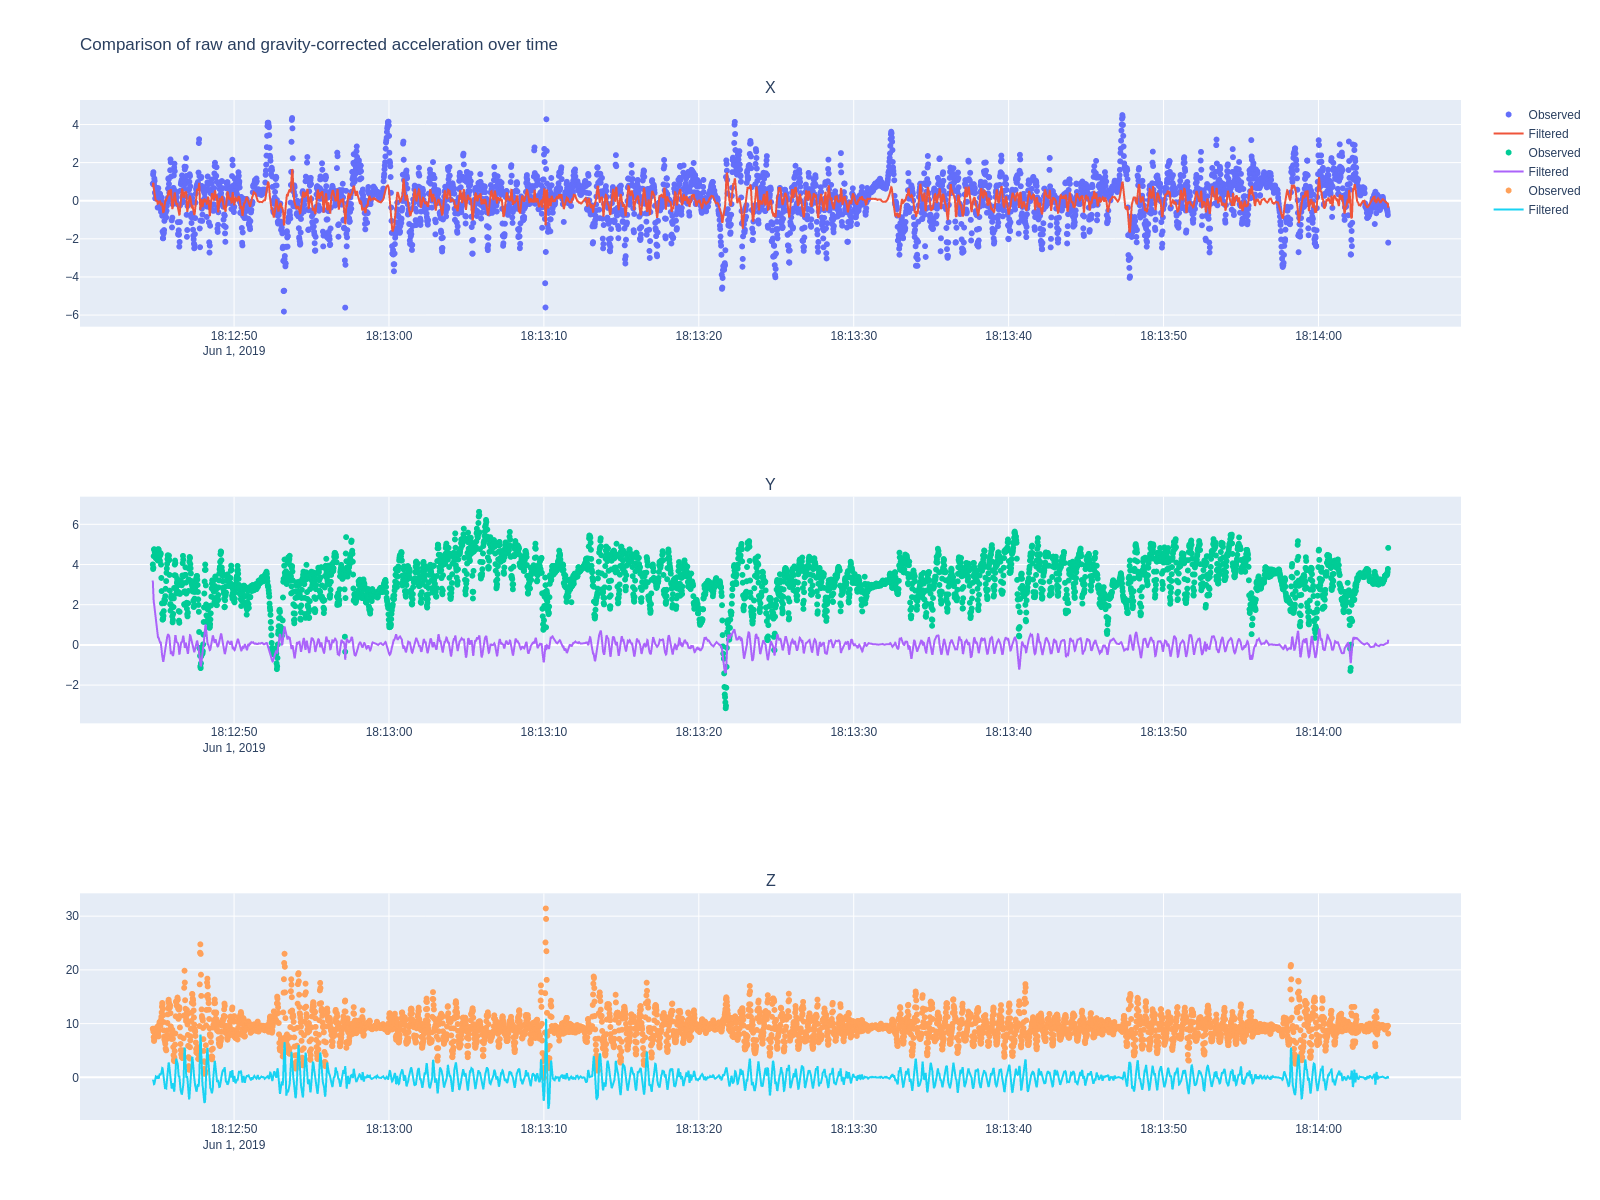
\includegraphics[width=300px]{figures/linear_accel.png}\\
    \caption{Comparison of raw and gravity-corrected acceleration over time}
    \label{fig:lin_accel}
\end{figure}

\subsubsection{Euler Angles}
Euler angles describe the orientation (pose) of a rigid body with respect to a reference coordinate frame
and can be estimated from a combination of the accelerometer and magnetometer data. The estimation of roll and pitch from sensed acceleration assumes that there is no linear acceleration at the start, and so any normalised accelerometer measurement can be related to gravitational acceleration through a rotation matrix \cite{aranburu2018imu}. The conversion from raw accelerometer readings to pose angle is shown in Equation \ref{eqn:psi} and \ref{eqn:theta}. 
  
\begin{equation} \label{eqn:psi}
    \psi_t = \tan^{-1} \left( \frac{\hat{\ddot{y_t}}}{\sqrt{\hat{\ddot{x_t}}^2 + \hat{\ddot{z_t}}}}\right)
\end{equation}
\begin{equation}\label{eqn:theta}
    \theta_t = \tan^{-1} \left( \frac{\hat{\ddot{x_t}}}{\sqrt{\hat{\ddot{y_t}}^2 + \hat{\ddot{z_t}}}}\right)
\end{equation}

These derived measurements are then used to transform the local magnetic field vectors into an estimate for the yaw angle. Magnetometer readings are defined in the body-fixed coordinate frame and so must undergo tilt compensation by rotating the sensor onto the horizontal plane \cite{jiang}.

\begin{equation}
    \zeta_x  = \begin{bmatrix}
        \(\cos{\theta_t}\)   \\
        \(\sin{\psi_t} \cdot \sin{\theta_t}\)   \\
        \(\cos{\psi_t} \cdot \sin{\theta_t}\)  \\
\end{bmatrix}  \begin{bmatrix}
        \(\hat \zeta_x\)   \\
        \(\hat \zeta_y\)   \\
        \(\hat \zeta_z\)  \\
\end{bmatrix}^T
\end{equation}

\begin{equation}
    \zeta_y  = \begin{bmatrix}
        0   \\
        \(\cos{\psi_t}\)   \\
        \(\sin{\psi_t}\)  \\
\end{bmatrix}  \begin{bmatrix}
        \(\hat \zeta_x\)   \\
        \(\hat \zeta_y\)   \\
        \(\hat \zeta_z\)  \\
\end{bmatrix}^T
\end{equation}

Where  \(\hat \zeta_x, \hat \zeta_y, and \hat \zeta_z\) are the raw magnetometer readings in the body frame. 
The yaw estimate can then be calculated as:
\begin{equation}
    \phi = \tan^{-1} \left( \frac{-\zeta_y}{\zeta_x}\right)
\end{equation}

\subsubsection{Euler Rates}
The gyroscope measures the angular velocity in the body-fixed reference frame. These Euler rates can then be derived from these measurements through a rotation into the world frame \cite{mathworks}. 

\begin{equation}
    \begin{bmatrix}
        \(\dot{\psi_t}\)   \\
        \(\dot{\theta_t}\)   \\
        \(\dot{\phi_t}\)  \\
\end{bmatrix}  = \begin{bmatrix}
        1 & \sin(\psi) \tan(\theta) & \cos(\psi) \tan(\theta)   \\
        1 & \cos(\psi) & -\sin(\psi)   \\
        1 & \frac{\sin(\psi)}{\cos(\theta)} & \frac{\cos(\psi)}{\cos(\theta)}   \\
\end{bmatrix}  \begin{bmatrix}
        \(\omega_x\)   \\
        \(\omega_y\)   \\
        \(\omega_z\)  \\
\end{bmatrix}
\end{equation}

\subsection{Control Input and Matrix}
No control inputs are factored into the state estimation and will therefore be omitted from the following analysis. 

\subsection{Measurement Matrix}
For this model, acceleration, pose and rotation rate are observed. This leads to the measurement matrix:

\begin{equation}
    H  = \begin{bmatrix}
        0 & 0 & 0 & 0 & 0 & 0 & 1 & 0 & 0 & 0 & 0 & 0 & 0 & 0 & 0 & 0 & 0 & 0 \\
        0 & 0 & 0 & 0 & 0 & 0 & 0 & 1 & 0 & 0 & 0 & 0 & 0 & 0 & 0 & 0 & 0 & 0  \\
        0 & 0 & 0 & 0 & 0 & 0 & 0 & 0 & 1 & 0 & 0 & 0 & 0 & 0 & 0 & 0 & 0 & 0  \\
        0 & 0 & 0 & 0 & 0 & 0 & 0 & 0 & 0 & 1 & 0 & 0 & 0 & 0 & 0 & 0 & 0 & 0  \\
        0 & 0 & 0 & 0 & 0 & 0 & 0 & 0 & 0 & 0 & 1 & 0 & 0 & 0 & 0 & 0 & 0 & 0  \\
        0 & 0 & 0 & 0 & 0 & 0 & 0 & 0 & 0 & 0 & 0 & 1 & 0 & 0 & 0 & 0 & 0 & 0  \\
        0 & 0 & 0 & 0 & 0 & 0 & 0 & 0 & 0 & 0 & 0 & 0 & 1 & 0 & 0 & 0 & 0 & 0  \\
        0 & 0 & 0 & 0 & 0 & 0 & 0 & 0 & 0 & 0 & 0 & 0 & 0 & 1 & 0 & 0 & 0 & 0  \\
        0 & 0 & 0 & 0 & 0 & 0 & 0 & 0 & 0 & 0 & 0 & 0 & 0 & 0 & 1 & 0 & 0 & 0  \\

\end{bmatrix} 
\end{equation}

\subsection{Process Noise Uncertainty Matrix}
Since the dynamic model doesn't include a control matrix, the process noise can be represented by the random variance in the accelerometer, gyroscope and magnetometer values.  This variance is derived from the sensor covariance, generated from the set of measurements across the full state space. The errors in the state are also interdependent, as values are some elements represent the integration of others over time. This relationship can be captured by defining the matrix $Q_s$ such that:

\begin{equation}
    Q_s  = \begin{bmatrix}
        \sigma_{a, x}^2 & 0 & 0 & 0 & 0 & 0 & 0 & 0 & 0 & 0 & 0 & 0 & 0 & 0 & 0 & 0 & 0 & 0 \\
        0 & \sigma_{a, y}^2 & 0 & 0 & 0 & 0 & 0 & 0 & 0 & 0 & 0 & 0 & 0 & 0 & 0 & 0 & 0 & 0 \\
        0 & 0 & \sigma_{a, z}^2 & 0 & 0 & 0 & 0 & 0 & 0 & 0 & 0 & 0 & 0 & 0 & 0 & 0 & 0 & 0 \\
        0 & 0 & 0 & \sigma_{a, x}^2 & 0 & 0 & 0 & 0 & 0 & 0 & 0 & 0 & 0 & 0 & 0 & 0 & 0 & 0 \\
        0 & 0 & 0 & 0 & \sigma_{a, y}^2 & 0 & 0 & 0 & 0 & 0 & 0 & 0 & 0 & 0 & 0 & 0 & 0 & 0 \\
        0 & 0 & 0 & 0 & 0 & \sigma_{a, z}^2 & 0 & 0 & 0 & 0 & 0 & 0 & 0 & 0 & 0 & 0 & 0 & 0 \\
        0 & 0 & 0 & 0 & 0 & 0 & \sigma_{a, x}^2 & 0 & 0 & 0 & 0 & 0 & 0 & 0 & 0 & 0 & 0 & 0 \\
        0 & 0 & 0 & 0 & 0 & 0 & 0 & \sigma_{a, y}^2 & 0 & 0 & 0 & 0 & 0 & 0 & 0 & 0 & 0 & 0  \\
        0 & 0 & 0 & 0 & 0 & 0 & 0 & 0 & \sigma_{a, z}^2 & 0 & 0 & 0 & 0 & 0 & 0 & 0 & 0 & 0  \\
        0 & 0 & 0 & 0 & 0 & 0 & 0 & 0 & 0 & \sigma_{g, x}^2 & 0 & 0 & 0 & 0 & 0 & 0 & 0 & 0  \\
        0 & 0 & 0 & 0 & 0 & 0 & 0 & 0 & 0 & 0 & \sigma_{g, y}^2 & 0 & 0 & 0 & 0 & 0 & 0 & 0  \\
        0 & 0 & 0 & 0 & 0 & 0 & 0 & 0 & 0 & 0 & 0 & \sigma_{g, z}^2 & 0 & 0 & 0 & 0 & 0 & 0  \\
        0 & 0 & 0 & 0 & 0 & 0 & 0 & 0 & 0 & 0 & 0 & 0 & \sigma_{g, x}^2 & 0 & 0 & 0 & 0 & 0  \\
        0 & 0 & 0 & 0 & 0 & 0 & 0 & 0 & 0 & 0 & 0 & 0 & 0 & \sigma_{g, y}^2 & 0 & 0 & 0 & 0  \\
        0 & 0 & 0 & 0 & 0 & 0 & 0 & 0 & 0 & 0 & 0 & 0 & 0 & 0 & \sigma_{m, z}^2 & 0 & 0 & 0  \\
        0 & 0 & 0 & 0 & 0 & 0 & 0 & 0 & 0 & 0 & 0 & 0 & 0 & 0 & 0 & \sigma_{g, x}^2 & 0 & 0 \\
        0 & 0 & 0 & 0 & 0 & 0 & 0 & 0 & 0 & 0 & 0 & 0 & 0 & 0 & 0 & 0 & \sigma_{g, y}^2 & 0 \\
        0 & 0 & 0 & 0 & 0 & 0 & 0 & 0 & 0 & 0 & 0 & 0 & 0 & 0 & 0 & 0 & 0 & \sigma_{m,z}^2 \\
\end{bmatrix}
\end{equation}

Where $\sigma_{a}$, $\sigma_{g}$ and $\sigma_{m}$ are the standard distribution of the accelerometer, gyroscope and magnetometer sensors respectively.

The interdependence of the state relationship can then be captured by Equation \ref{eqn:Q}, thereby better representing the noise inherent in the dynamic model \cite{kalmanfilternet}.

\begin{equation} \label{eqn:Q}
    \bold{Q} = \bold{A}\bold{Q_s}\bold{A}^T
\end{equation}


\section{Kalman Filter Algorithm}
\subsection{Process}
The Kalman Filter algorithm learns the dynamics of the state space through recursively minimising a quadratic cost function with respect to the estimated spaced and the correct space. This process consists of two primary phases: the predict and the update phase.

The predict phase uses knowledge of the state transition dynamics and the inherent noise characteristics to estimate the state and estimate uncertainty at time $t + 1$. Assuming the system we are modelling is linear, the discrete model can be written as:

\begin{equation}
    X_{t, p} = AX_{t-1} + w_{t}
\end{equation}

Where $X_{t, p}$ is the state estimate and $w_{t}$ is white Gaussian noise. 

\begin{equation}
    P_{t, p} = AP_{t-1}A^T + Q
\end{equation}

The update phase is triggered by the input of a new observation and measurement uncertainty into the system and updates the state such that the uncertainty of future predictions is minimised. This update consists of the following equations:

\begin{equation}
    K_t = \frac{P_{t, p}H^t}{HP_{t, p}H^T + R}
\end{equation}
Where $K_t$ is the Kalman gain, and R is the measurement uncertainty matrix.

\begin{equation}
    X_t = X_{t, p} + K_t [Y_t - H X_t]
\end{equation}

Where $X_t$ is the estimated state space. 

\begin{equation}
    P_k = (I - K_t H)P_{t, p}
\end{equation}

Where $P_k$ is the estimated uncertainty and I is the identity matrix.

If the process inputs fully represent the state space, the Kalman gain and estimate uncertainty should converge towards zero over time.

\subsection{Initial Conditions}

The initial state estimate is given by the initial waypoint location and linear acceleration. All other values are estimated to be zero.

\begin{equation} 
X_0 =  \begin{bmatrix}
        x_0  \\
        y_0 \\
        z_0   \\
        0  \\ 
        0   \\
        0  \\
        \(\ddot x_t\)   \\
        \(\ddot y_t\)   \\
        \(\ddot z_t\)  \\
        0  \\
        0  \\
        0   \\
        0  \\ 
        0   \\
        0   \\
        0  \\ 
        0   \\
        0   \\
\end{bmatrix} 
\end{equation}

As the initial state is highly uncertain, the initial estimate uncertainty is set to an arbitrarily large value. In this case, the estimate uncertainty was represented by:

\begin{equation} 
P_0 = I\cdot500  
\end{equation}

\section{Evaluation}

The Kalman Filter was modelled in python and run across numerous test data sets to evaluate the efficacy of this model. Overall, the model consistently showed convergence over time for a majority of the state element, with some notable exceptions. Comparing the observable state elements in Figures \ref{fig:acc}, \ref{fig:euler}, and \ref{fig:rate}, there is a significant decrease in the noise of the filtered data compared with the derived observations. 

\begin{figure}[H]
    \centering
    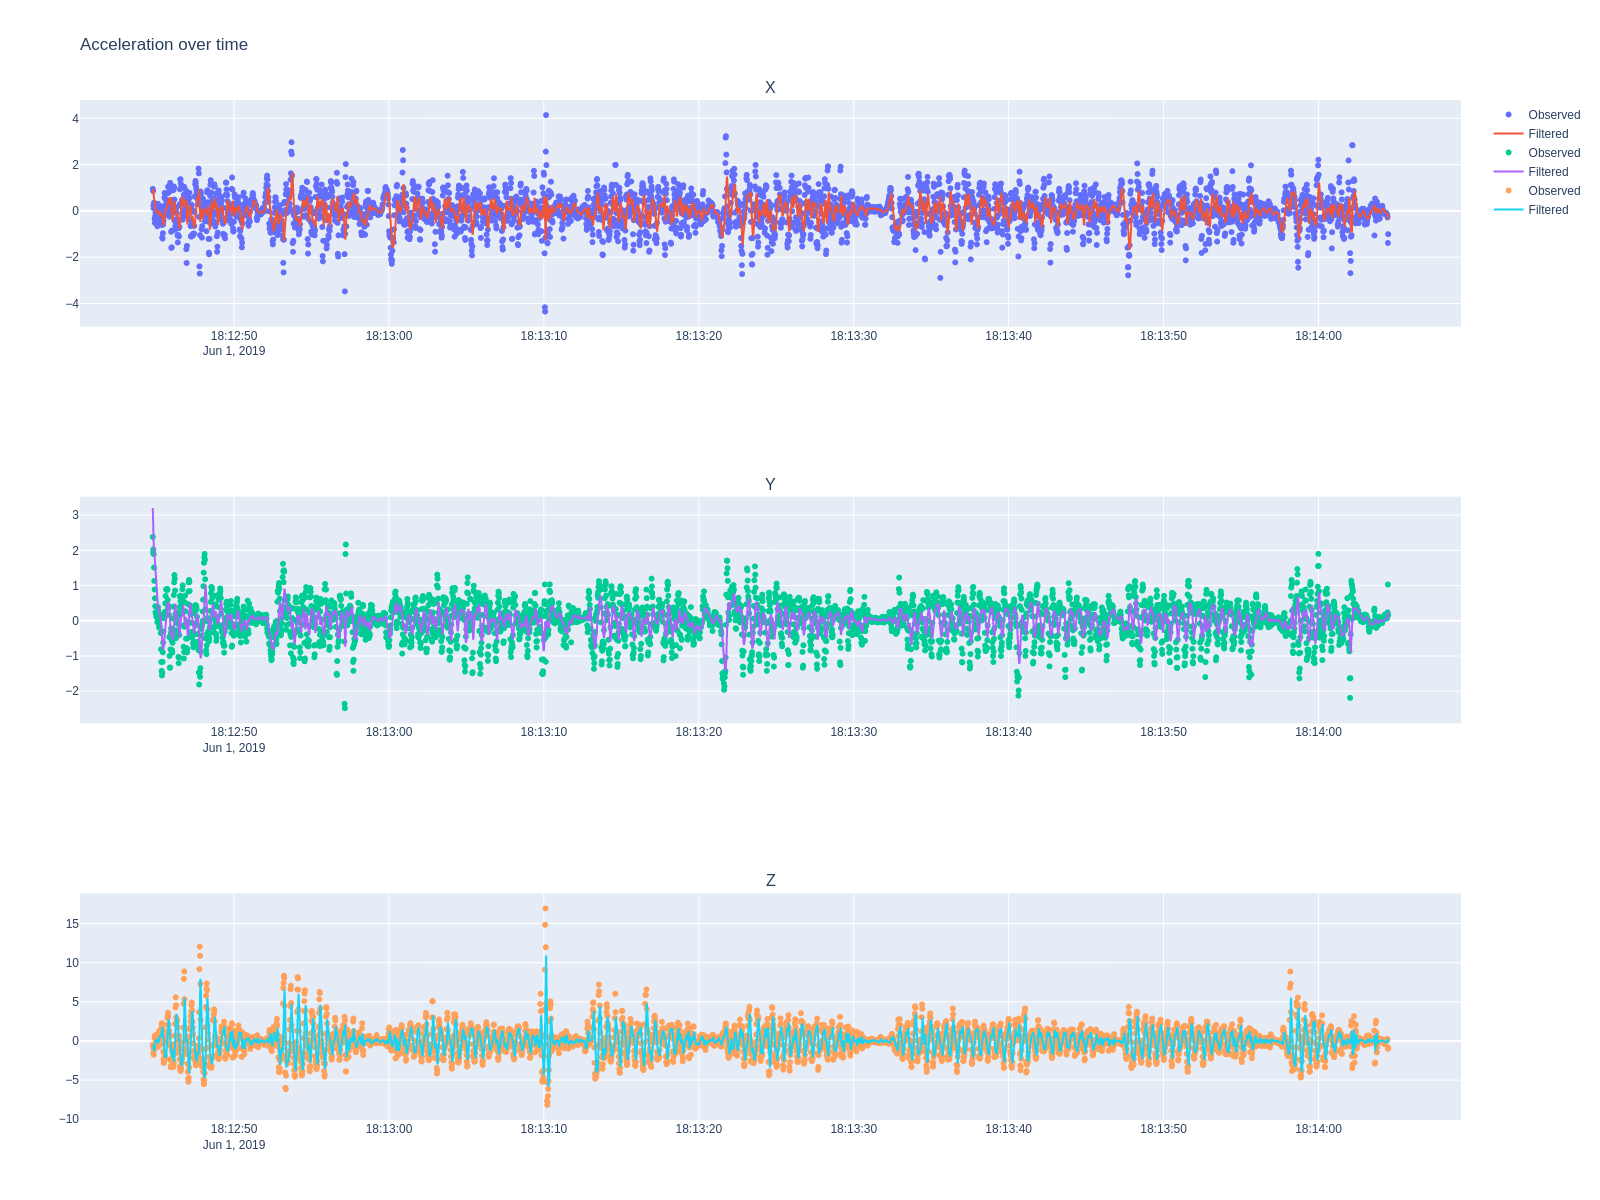
\includegraphics[width=300px]{figures/acc_obs_comparison.png}\\
    \caption{Comparison of raw and filtered acceleration  over time}
    \label{fig:acc}
\end{figure}

\begin{figure}[H]
    \centering
    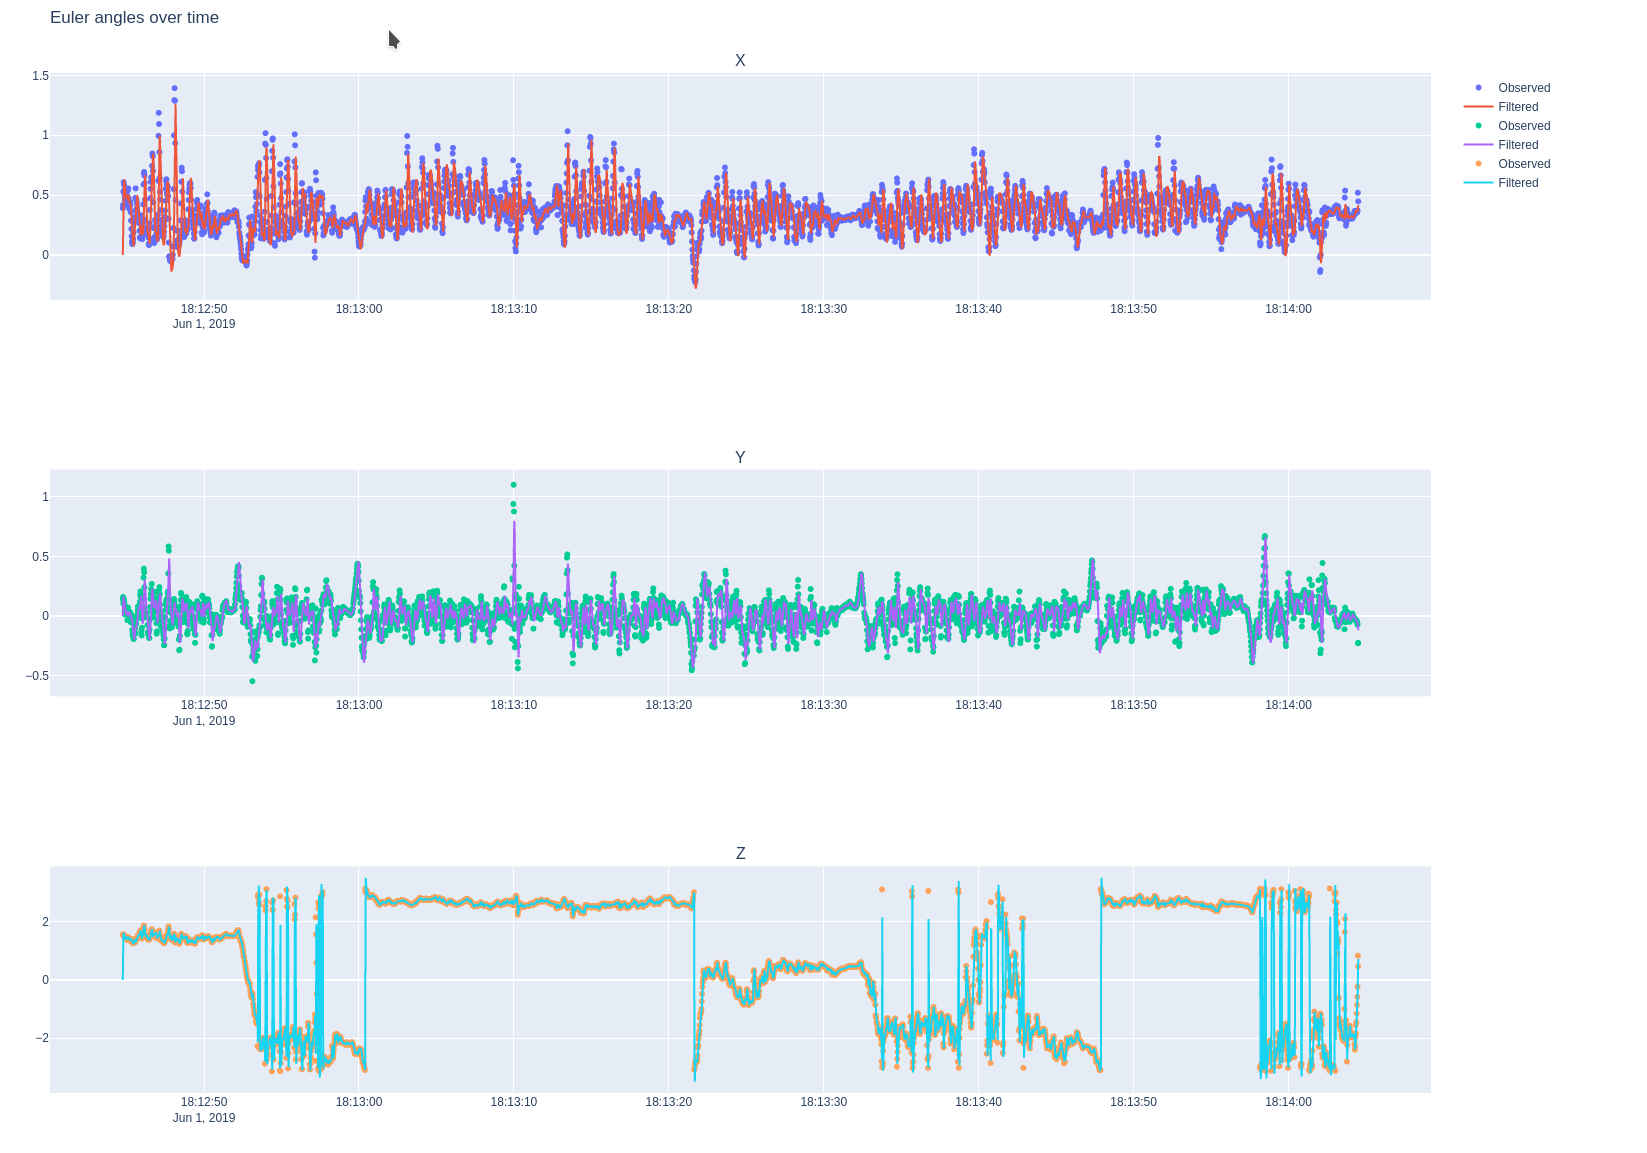
\includegraphics[width=300px]{figures/eul_obs_comparison.png}\\
    \caption{Comparison of raw and filtered Euler angles  over time}
    \label{fig:euler}
\end{figure}
\begin{figure}[H]
    \centering
    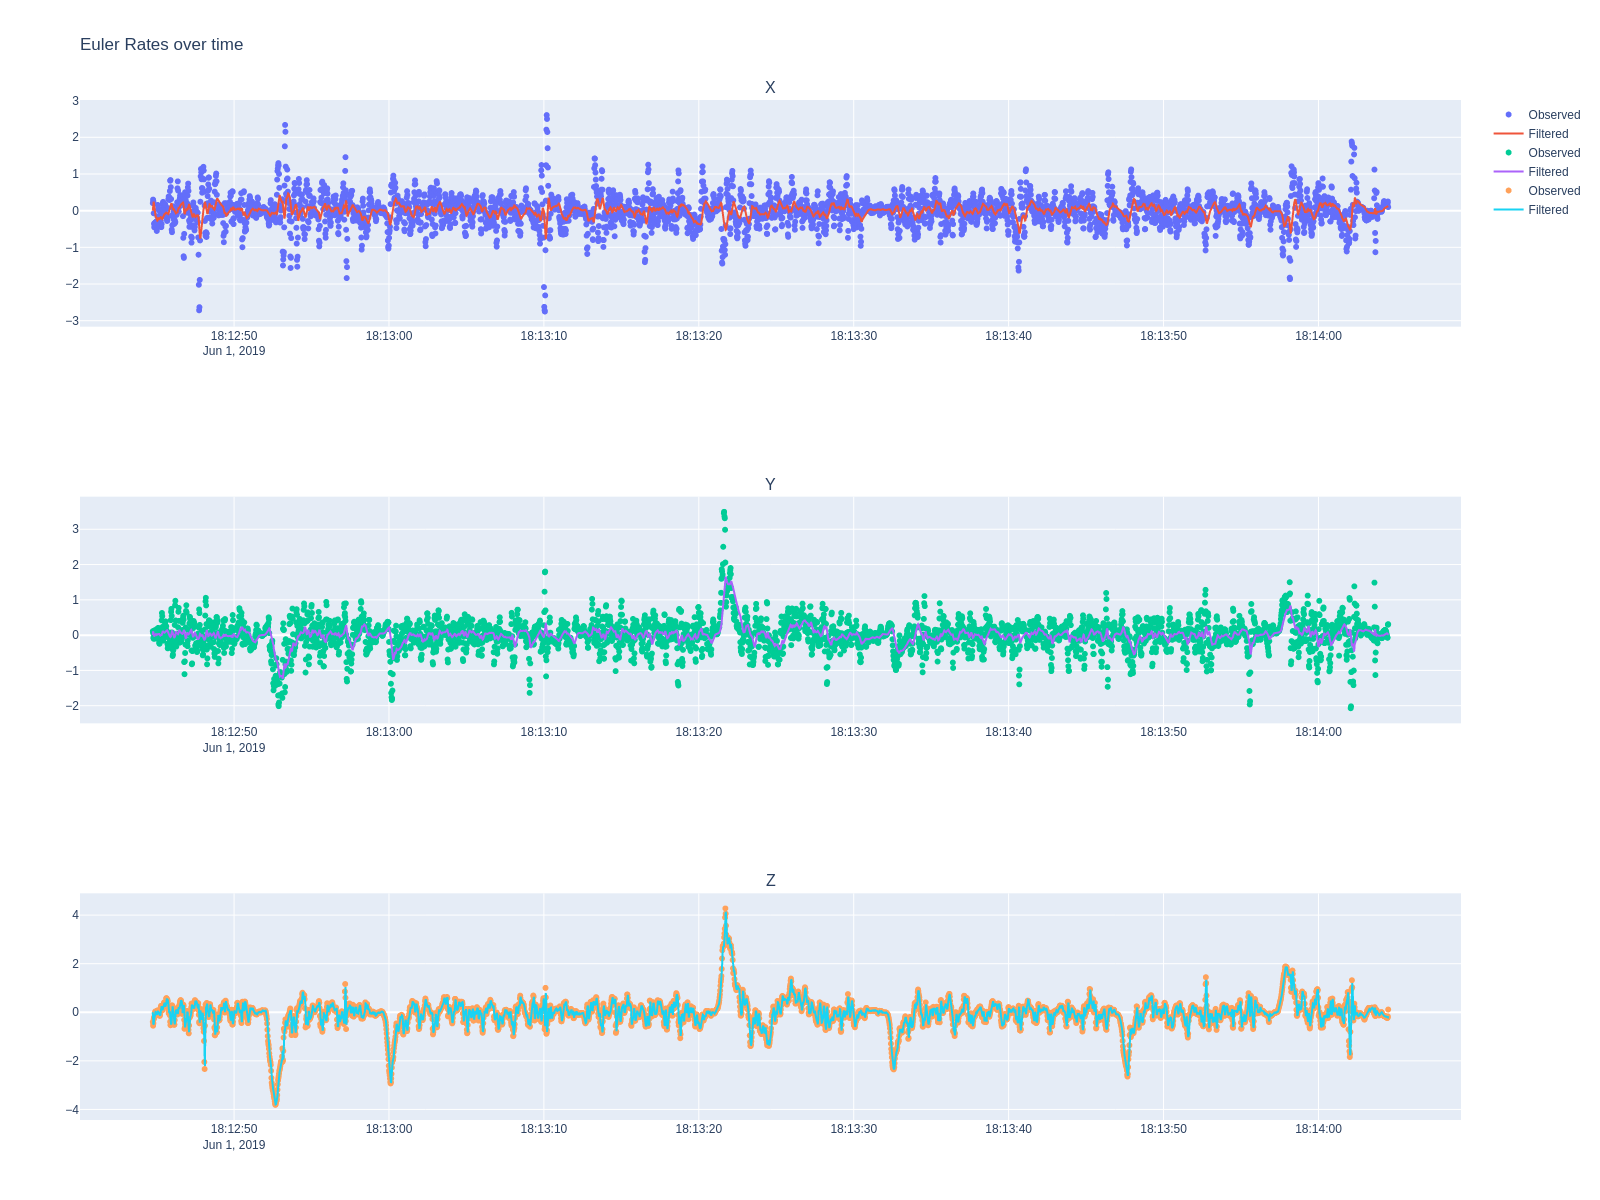
\includegraphics[width=300px]{figures/eulr_obs_comparison.png}\\
    \caption{Comparison of raw and filtered Euler rates  over time}
    \label{fig:rate}
\end{figure}

Figure \ref{fig:gain} displays the steady decrease in Kalmain gain for acceleration over time, suggesting that the model's predicted state became a more accurate representation of the true state than the noisy measurement data. 

\begin{figure}[H]
    \centering
    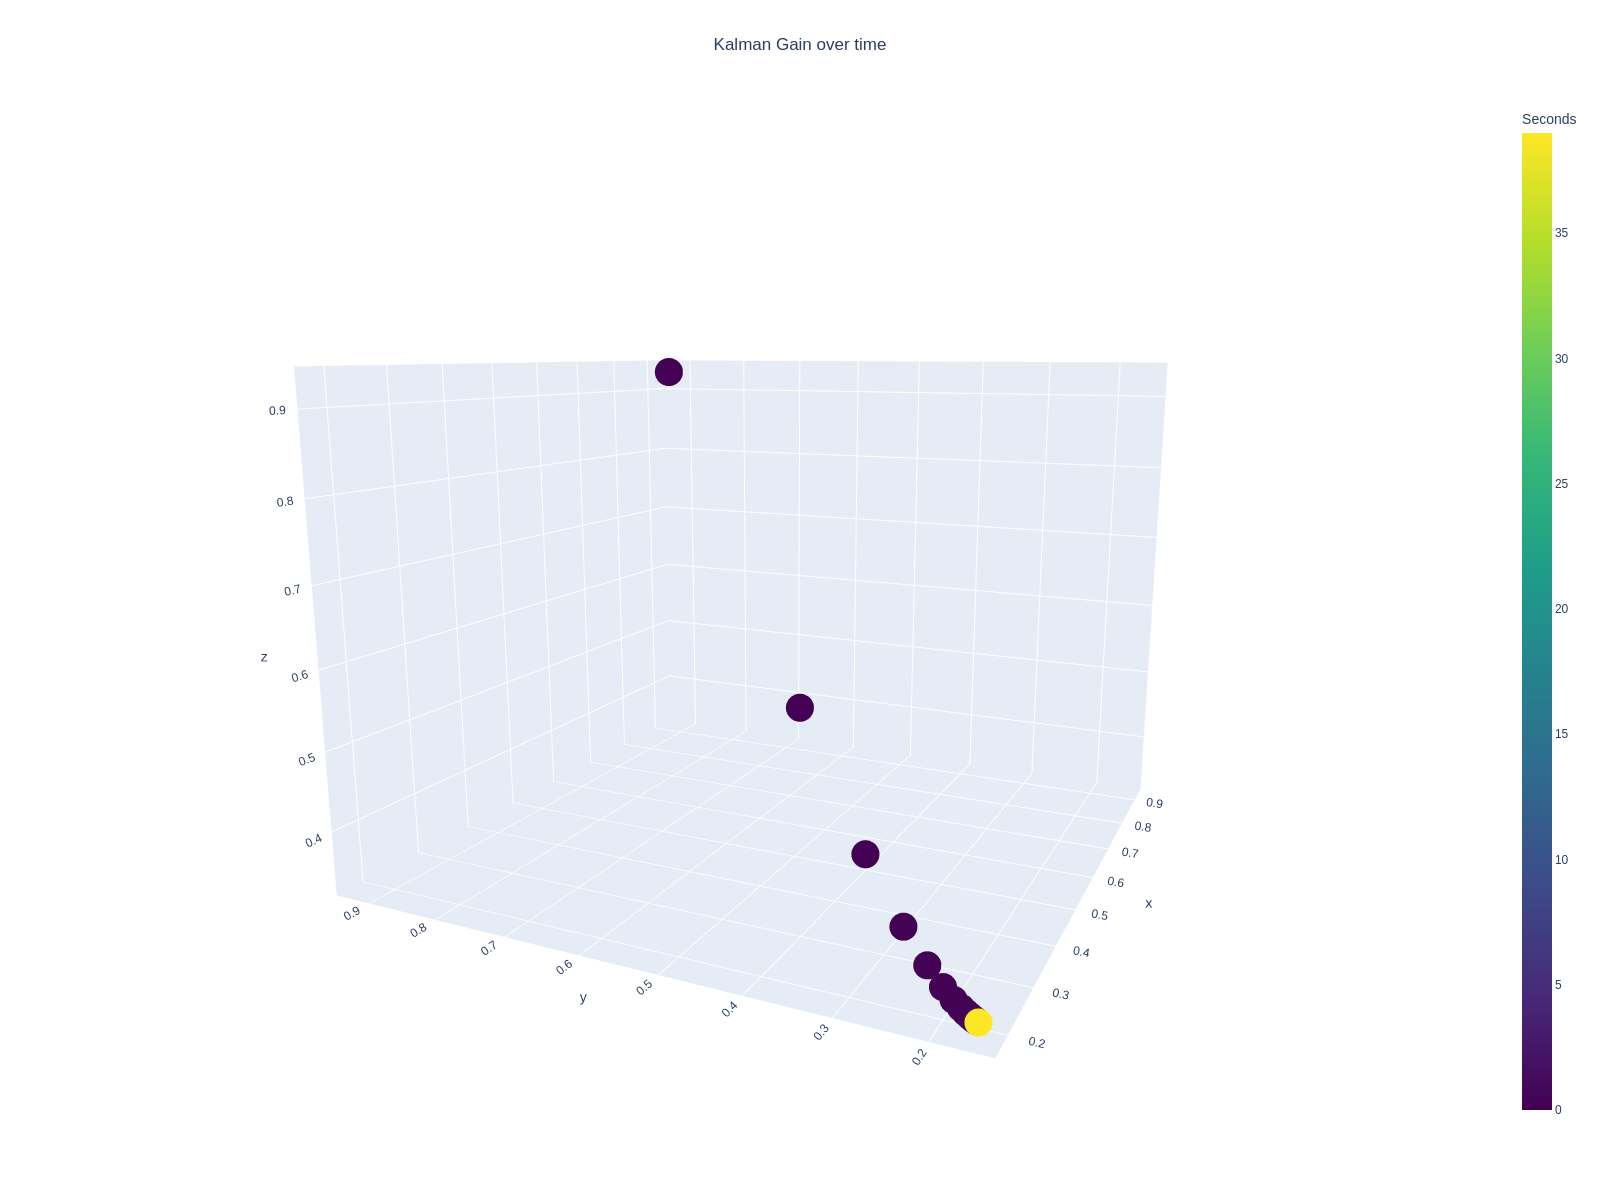
\includegraphics[width=300px]{figures/kalman_gain.png}\\
    \caption{Kalmain Gain convergence over time}
    \label{fig:gain}
\end{figure}

Therefore, the model can be shown to perform well for the state elements that can be validated against measurable data. However, Figure \ref{fig:pos} displays the performance of the estimated position against the true value, derived from the list of waypoints. The model shows clear divergence from the source truth, and fails to replicate trends the robot takes along the path. This degraded performance can clearly be seen in Figures \ref{fig:x} to \ref{fig:vz}, where the uncertainty displays an unbounded increase over time. This can likely be attributed to errors in the acceleration estimate compounding, as the model has no means with which to refine the predictions over time.  An improvement to the model could therefore be the addition of GPS data, which would provide information about the current position of the vehicle in an external reference frame. 
\begin{figure}[H]
    \centering
    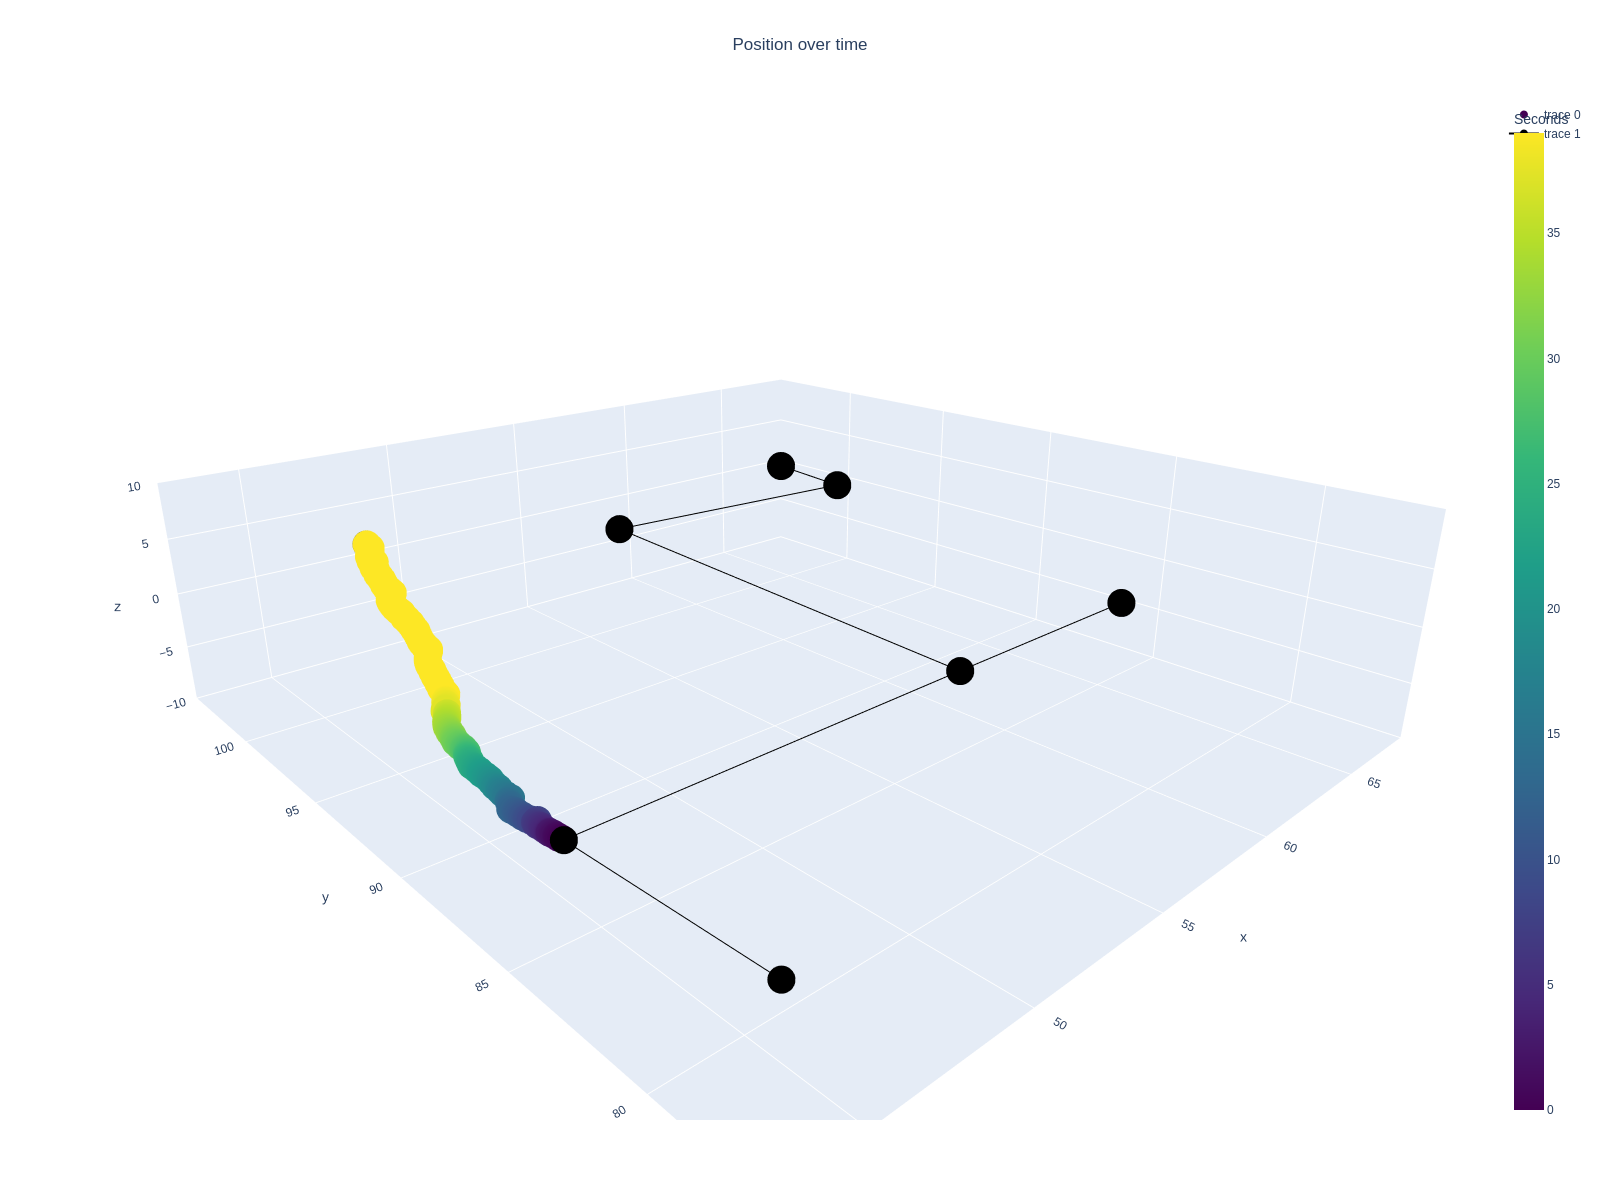
\includegraphics[width=300px]{figures/position.png}\\
    \caption{3D Position over time}
    \label{fig:pos}
\end{figure}

Figure \ref{fig:pos2} shows a similar divergence from the true value, but shows a closer approximation of the path and terminates near the final waypoint. 

\begin{figure}[H]
    \centering
    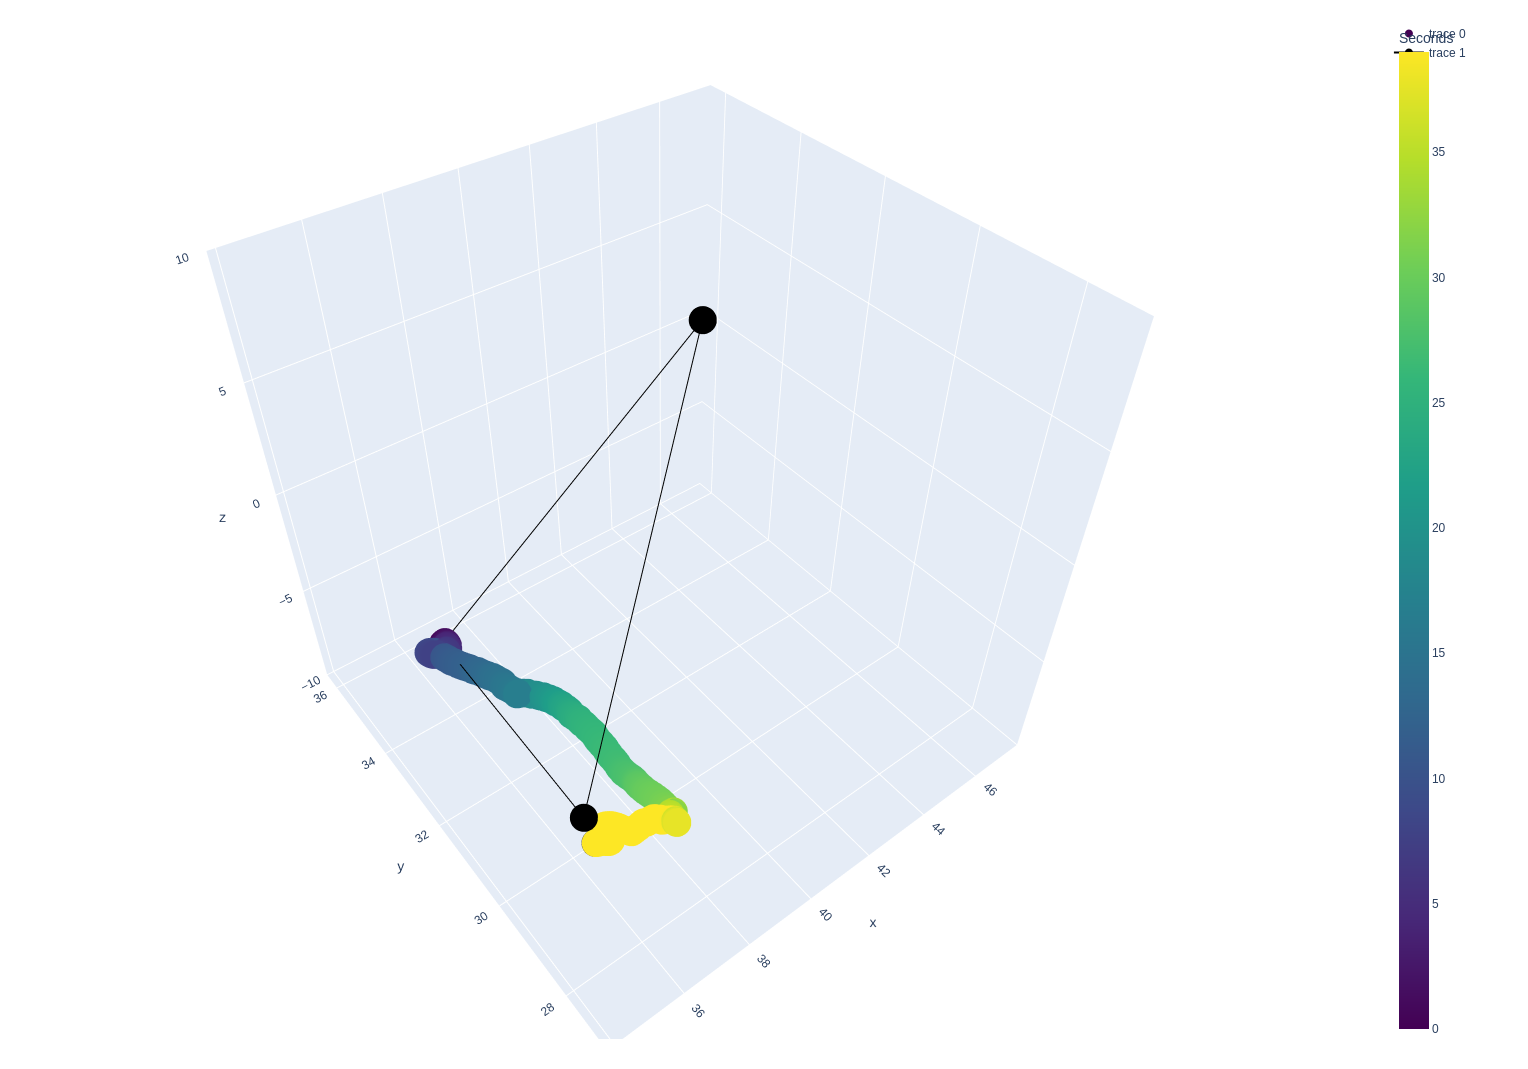
\includegraphics[width=300px]{figures/path2.png}\\
    \caption{3D Position over time for alternate data set}
    \label{fig:pos2}
\end{figure}


Another notable feature of the model is that the roll, pitch and yaw biases can be seen to converge over time, with roll and pitch rapidly converging towards zero. In comparison, though yaw bias does not exhibit unbounded uncertainty growth, the values oscillate around a non-zero value, indicating an unstable estimate function. This is further seen in Figure \ref{fig:euler}, where the estimates poorly track the noisy data. A possible explanation for this is its derivation from magnetometer readings, a sensor that is easily perturbed by  electromagnetic disturbances from hard iron, electric current and indoor environments \cite{wu2019real}. 

A key parameter of the model is the initial estimate uncertainty, as it is will affect the degree to which the Kalman Filter will weight the model prediction against the measurements. Too low an inital uncertainty, and the model can fail to converge to the true representation of the stare. In Figure \ref{fig:gain_u}, a low uncertainty for the uncertain initial estimate results in a diverging Kalman gain over time and unstable uncertainties for state estimates.

\begin{figure}[H]
    \centering
    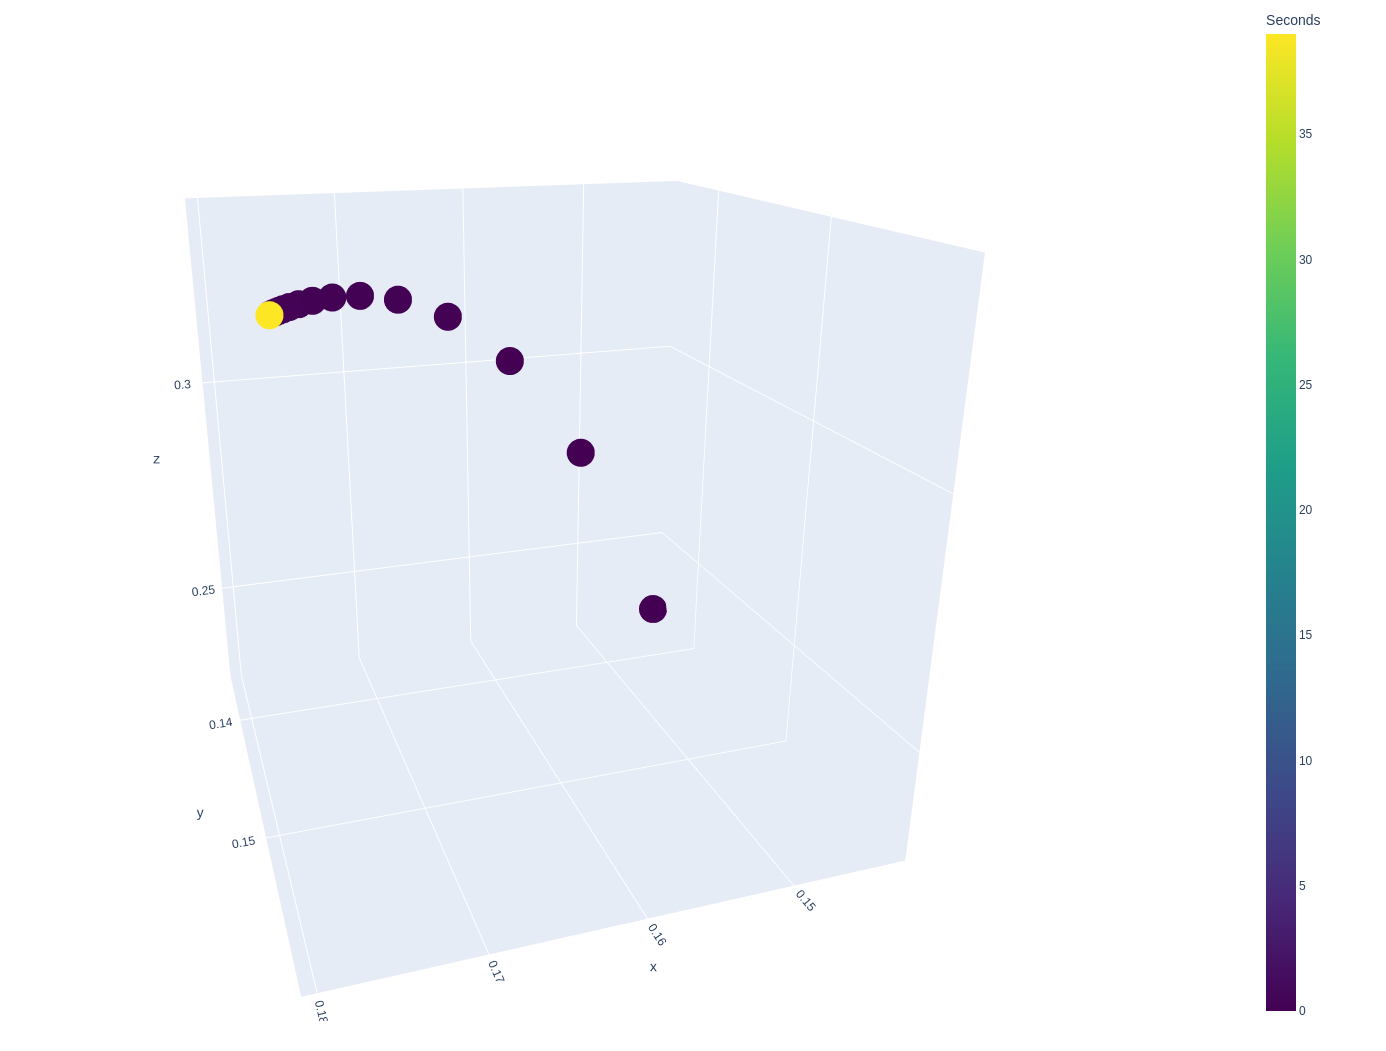
\includegraphics[width=300px]{figures/kalman_gain_low_uncertainty.png}\\
    \caption{Kalman Gain divergence over time from low initial uncertainty}
    \label{fig:gain_u}
\end{figure}

\section{Conclusion}
Though the linear Kalman filter is generally considered to be a poor estimator for non-linear state spaces, the model output reasonable estimates for most state elements despite the complexity of the system. The model clearly showed convergence towards a stable estimate for the state space that was a reasonable approximation of the noisy data. It is recommended that non-linear Kalman filter algorithms, such as EKFs or UKFs are considered, to identify if uncertainties in the position, velocity and yaw derivatives can be minimised. 

\newpage
%======Though the===========================================================
%                           List of Figures
%=================================================================
\section{List of Figures}
\lhead{Figures} % section header

\begin{figure}[H]
    \centering
    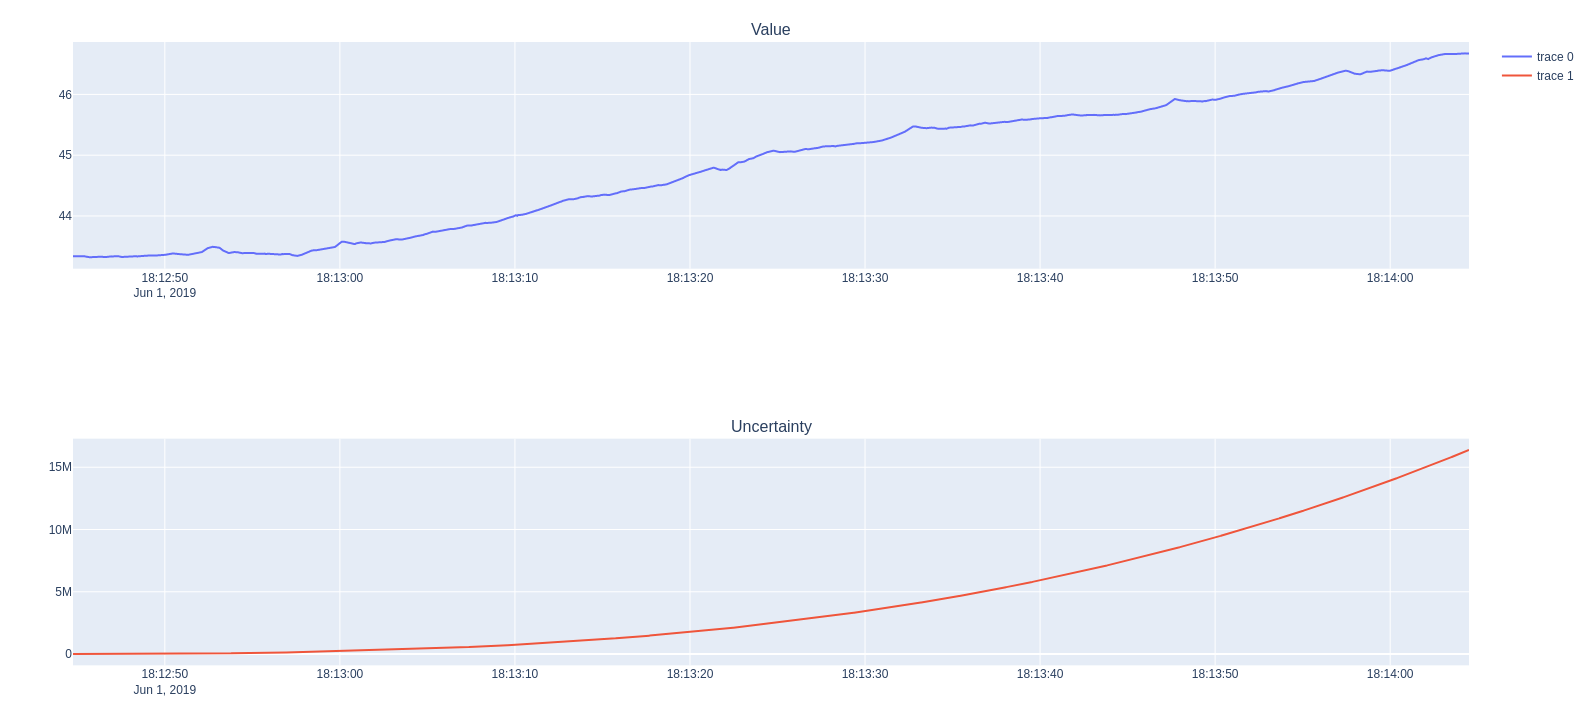
\includegraphics[width=\linewidth]{figures/x_uncertainty.png}\\
    \caption{X Position state and uncertainty over time}
    \label{fig:x}
\end{figure}
\begin{figure}[H]
    \centering
    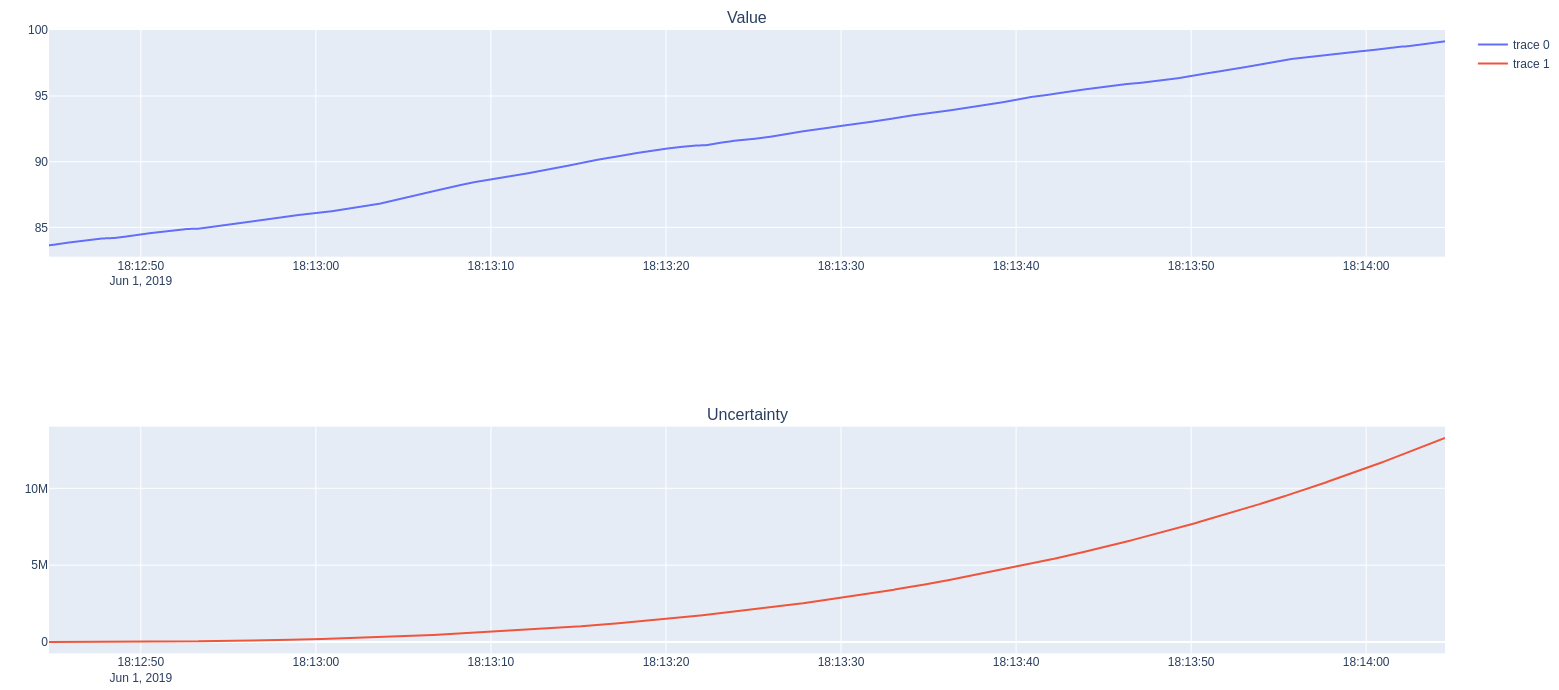
\includegraphics[width=\linewidth]{figures/y_uncertainty.png}\\
    \caption{Y Position state and uncertainty over time}
    \label{fig:y}
\end{figure}

\begin{figure}[H]
    \centering
    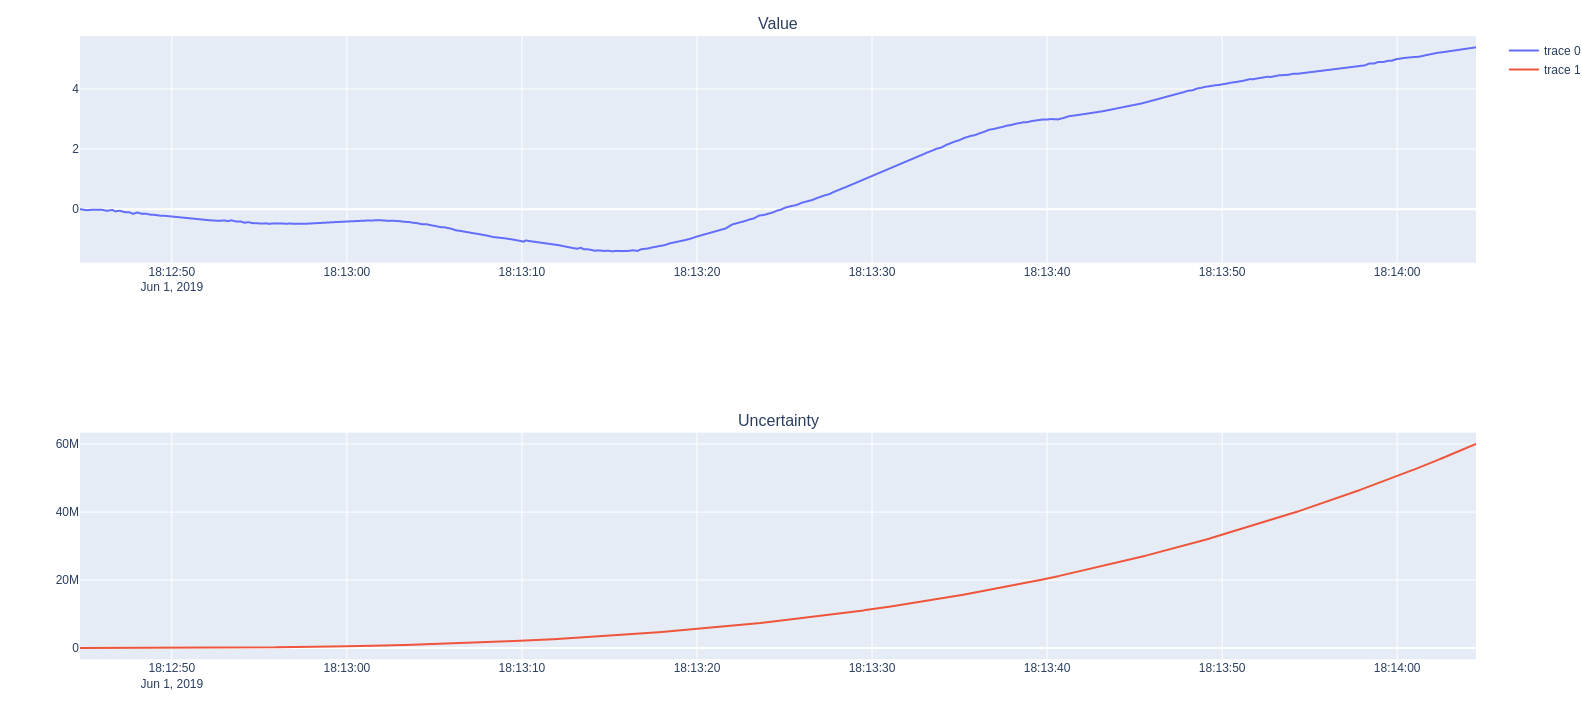
\includegraphics[width=\linewidth]{figures/z_uncertainty.png}\\
    \caption{Z Position state and uncertainty over time}
    \label{fig:z}
\end{figure}

\begin{figure}[H]
    \centering
    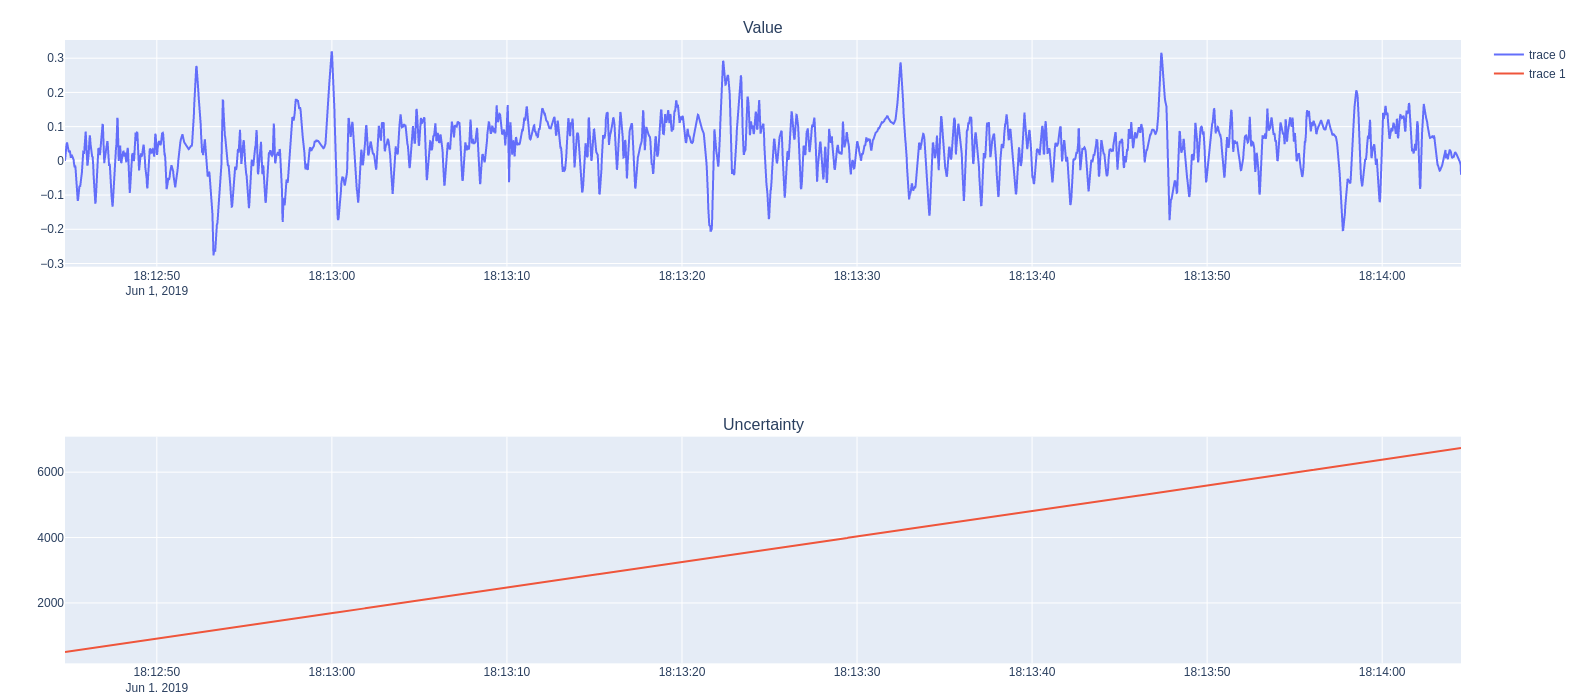
\includegraphics[width=\linewidth]{figures/vx_uncertainty.png}\\
    \caption{X Velocity state and uncertainty over time}
    \label{fig:vx}
\end{figure}
\begin{figure}[H]
    \centering
    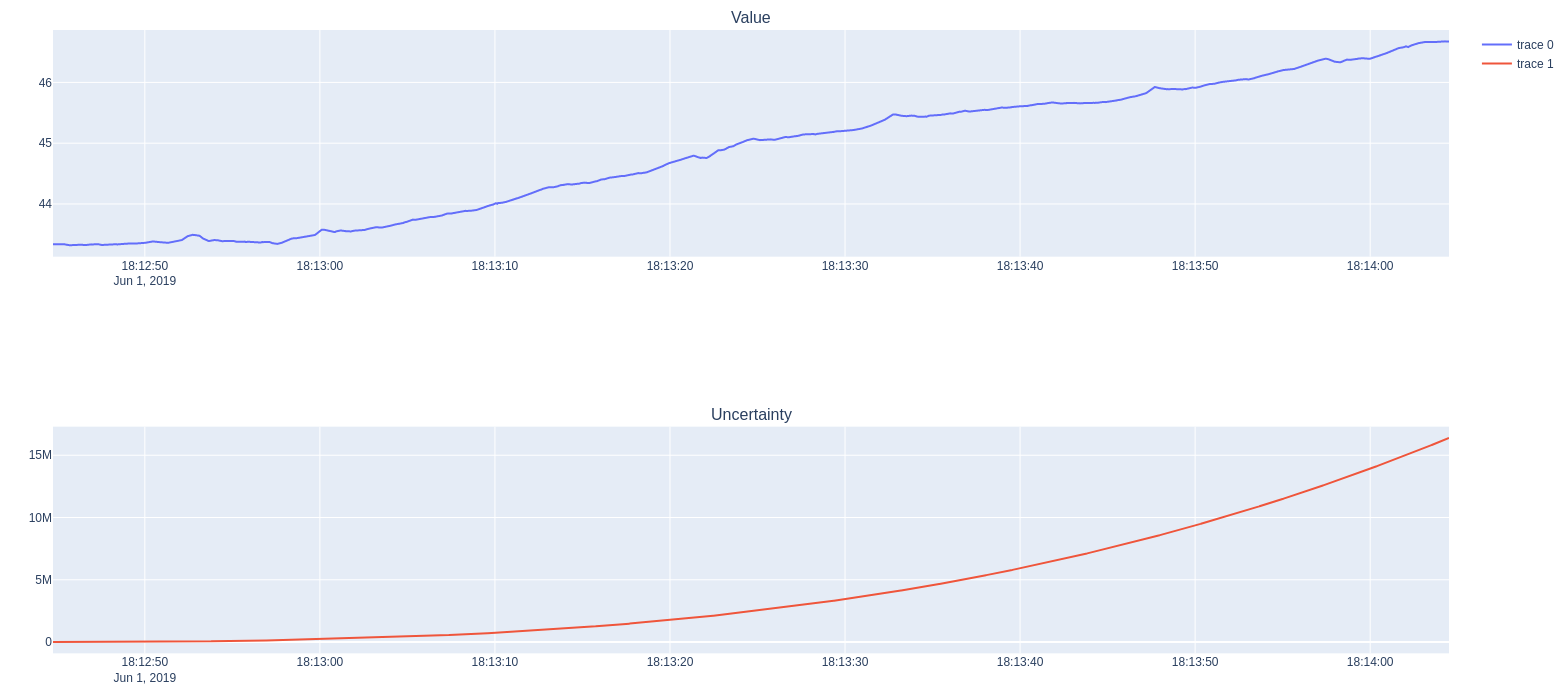
\includegraphics[width=\linewidth]{figures/vy_uncertainty.png}\\
    \caption{Y Velocity state and uncertainty over time}
    \label{fig:vy}
\end{figure}
\begin{figure}[H]
    \centering
    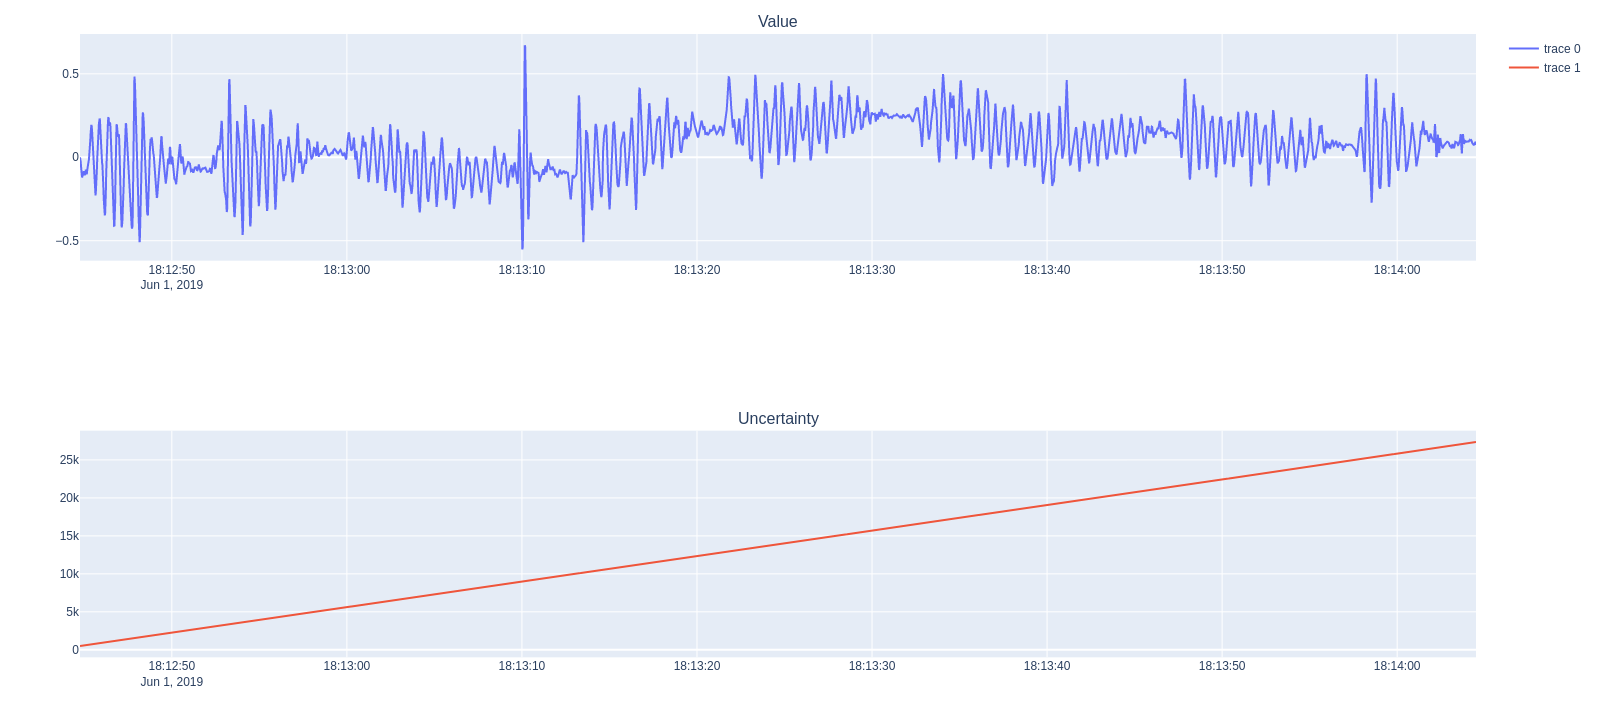
\includegraphics[width=\linewidth]{figures/vz_uncertainty.png}\\
    \caption{Z Velocity state and uncertainty over time}
    \label{fig:vz}
\end{figure}

\begin{figure}[H]
    \centering
    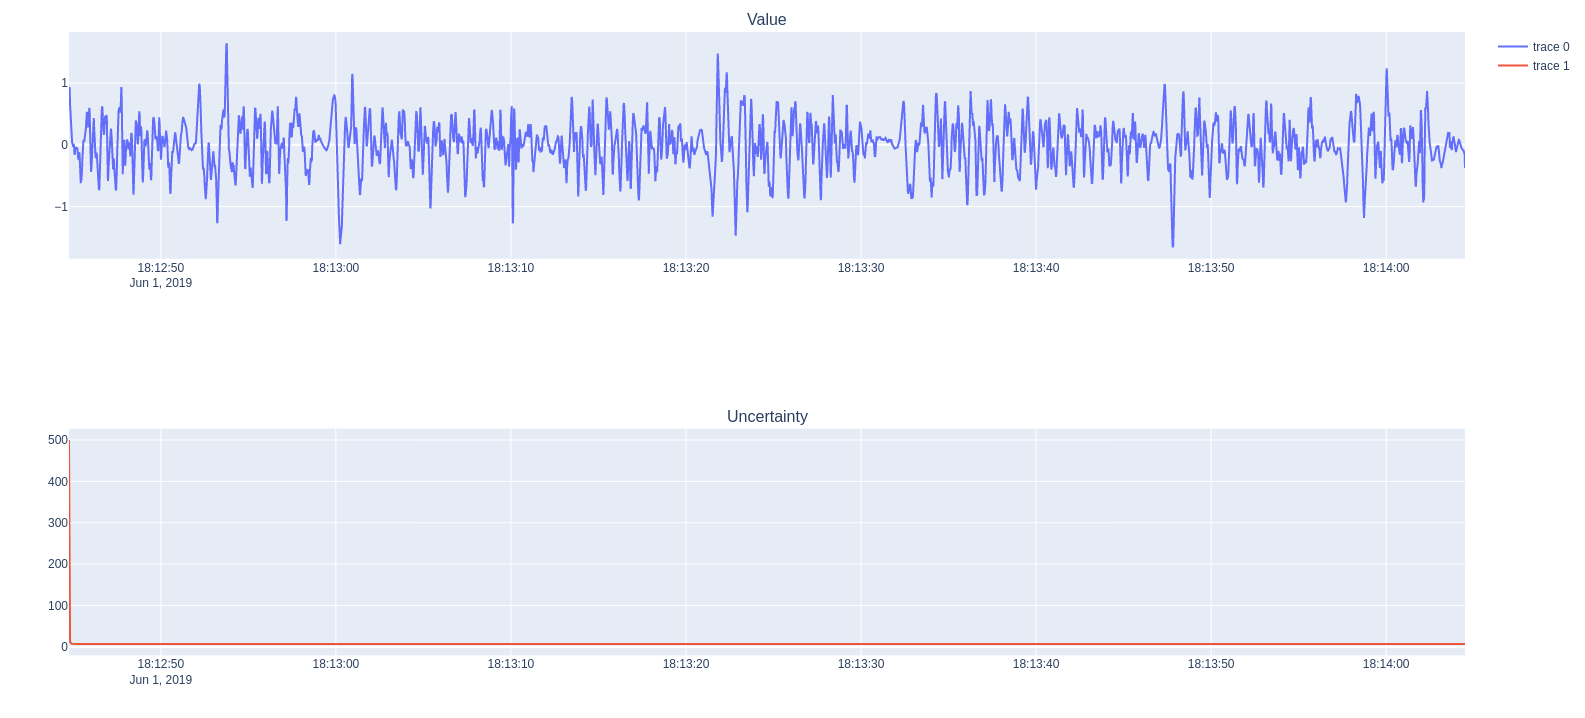
\includegraphics[width=\linewidth]{figures/ax_uncertainty.png}\\
    \caption{X Acceleration state and uncertainty over time}
    \label{fig:az}
\end{figure}
\begin{figure}[H]
    \centering
    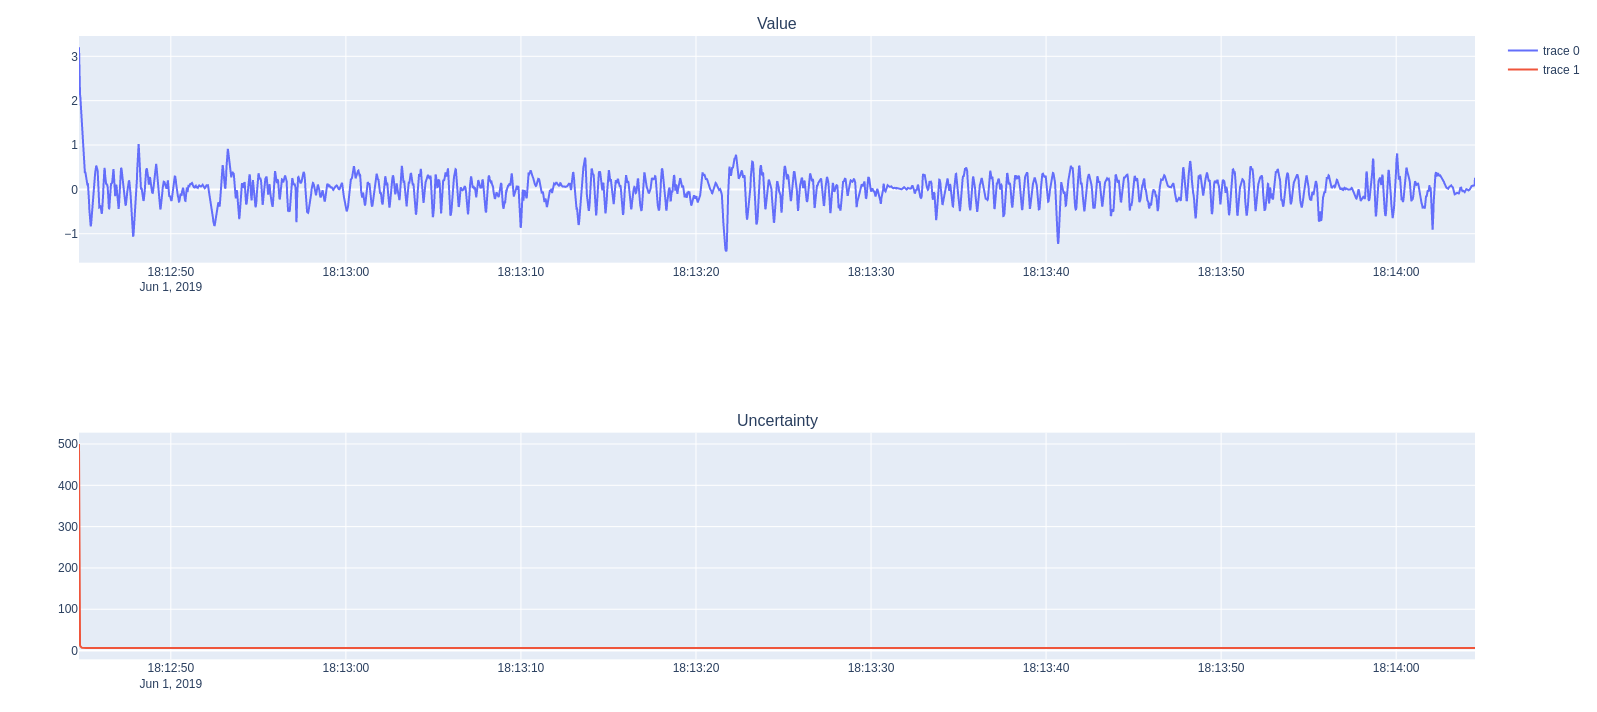
\includegraphics[width=\linewidth]{figures/ay_uncertainty.png}\\
    \caption{Y Acceleration state and uncertainty over time}
    \label{fig:ay}
\end{figure}
\begin{figure}[H]
    \centering
    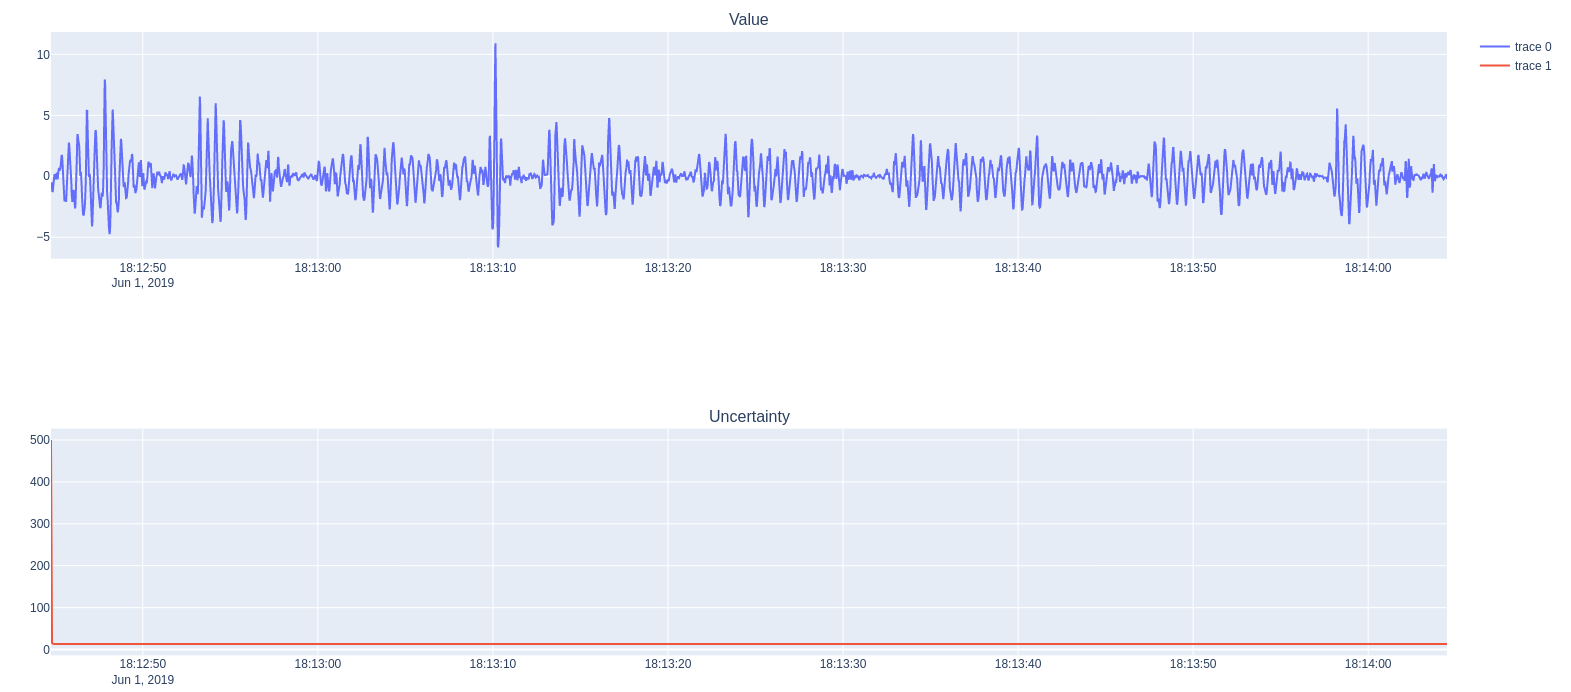
\includegraphics[width=\linewidth]{figures/az_uncertainty.png}\\
    \caption{Z Acceleration state and uncertainty over time}
    \label{fig:az}
\end{figure}

\begin{figure}[H]
    \centering
    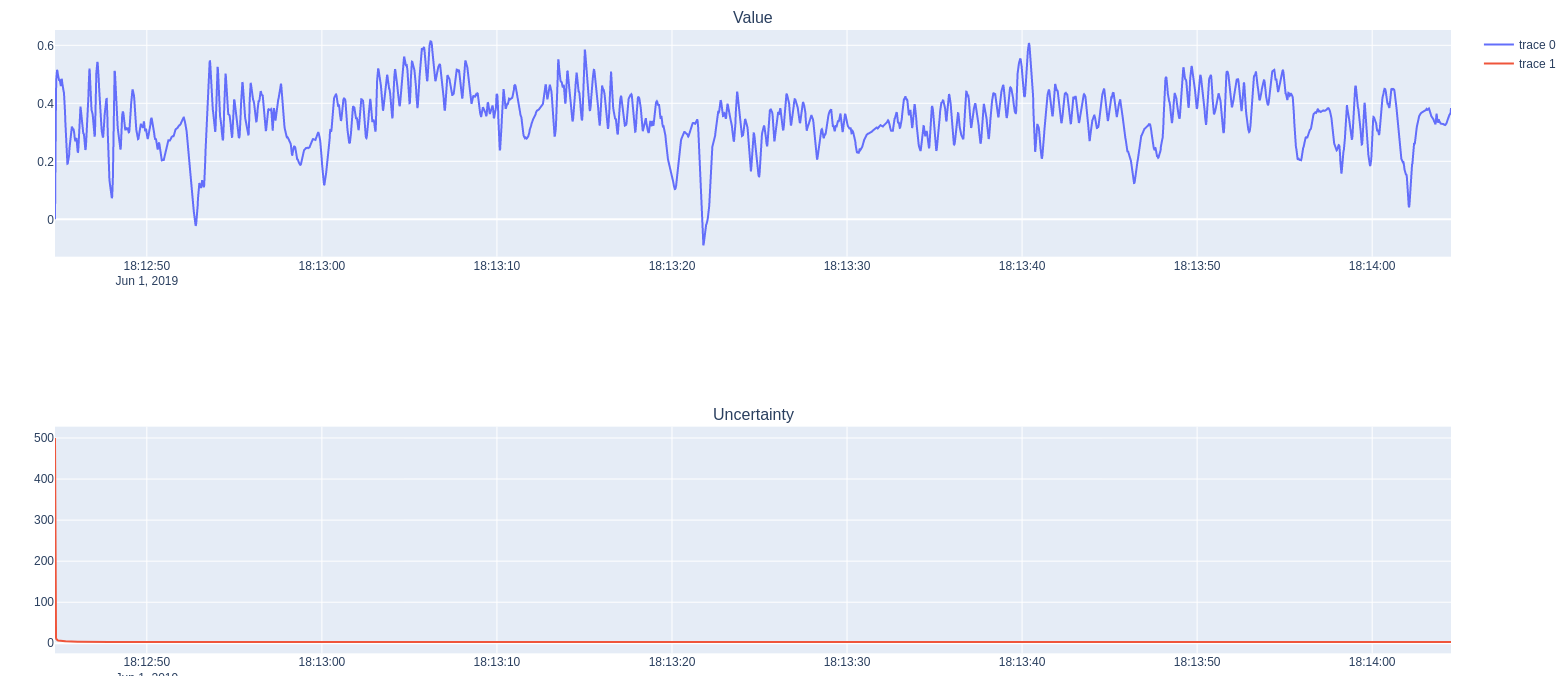
\includegraphics[width=\linewidth]{figures/r_uncertainty.png}\\
    \caption{Roll state and uncertainty over time}
    \label{fig:r}
\end{figure}
\begin{figure}[H]
    \centering
    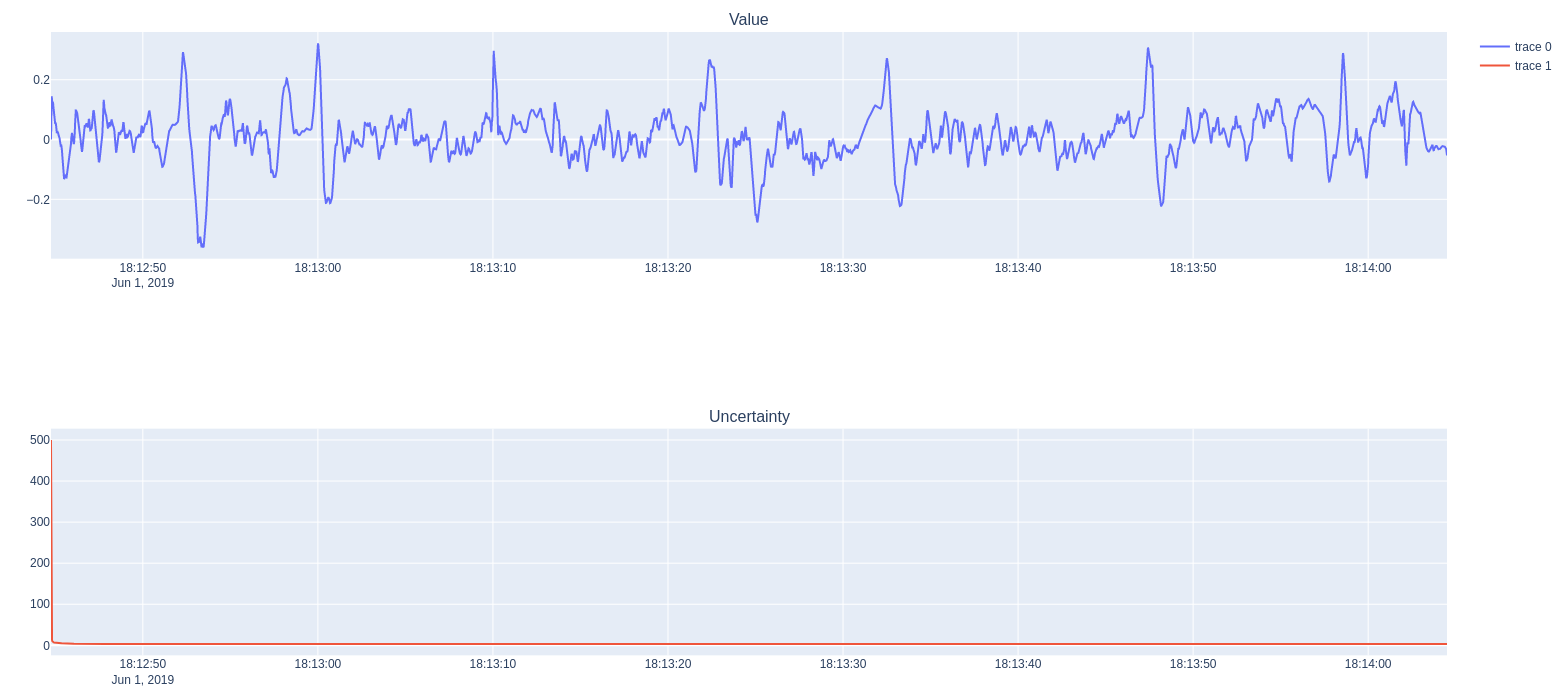
\includegraphics[width=\linewidth]{figures/p_uncertainty.png}\\
    \caption{Pitch state and uncertainty over time}
    \label{fig:p}
\end{figure}
\begin{figure}[H]
    \centering
    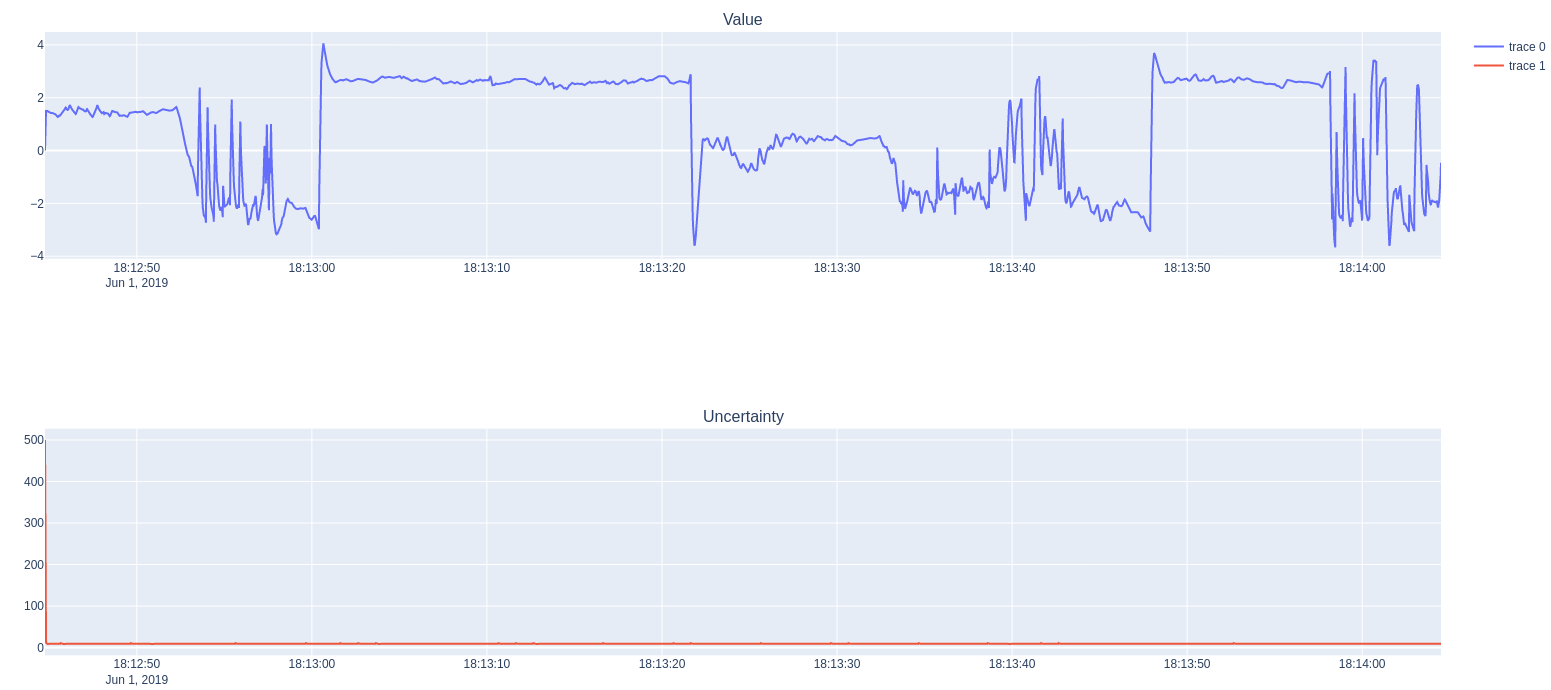
\includegraphics[width=\linewidth]{figures/yw_uncertainty.png}\\
    \caption{Yaw state and uncertainty over time}
    \label{fig:yw}
\end{figure}

\begin{figure}[H]
    \centering
    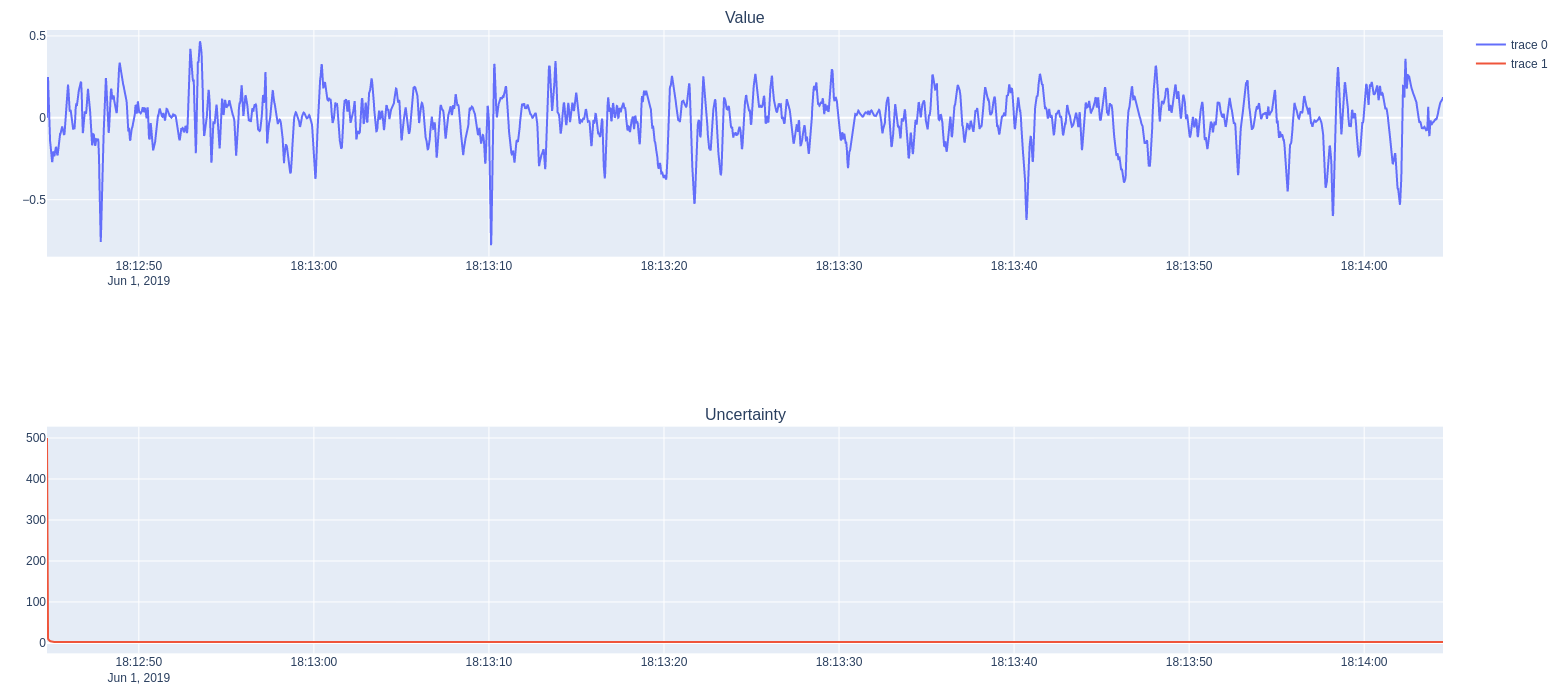
\includegraphics[width=\linewidth]{figures/vr_uncertainty.png}\\
    \caption{Roll rate state and uncertainty over time}
    \label{fig:vr}
\end{figure}
\begin{figure}[H]
    \centering
    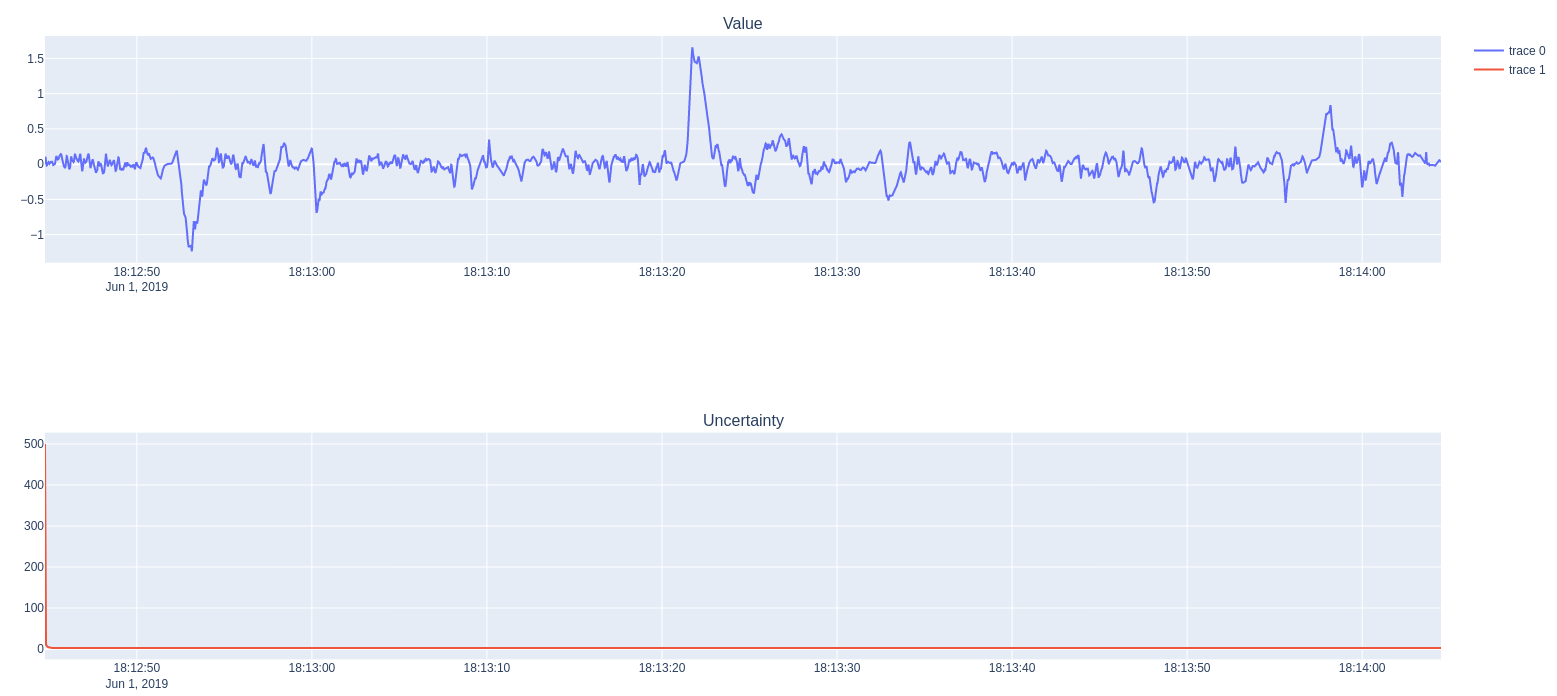
\includegraphics[width=\linewidth]{figures/vp_uncertainty.png}\\
    \caption{Pitch rate state and uncertainty over time}
    \label{fig:vp}
\end{figure}
\begin{figure}[H]
    \centering
    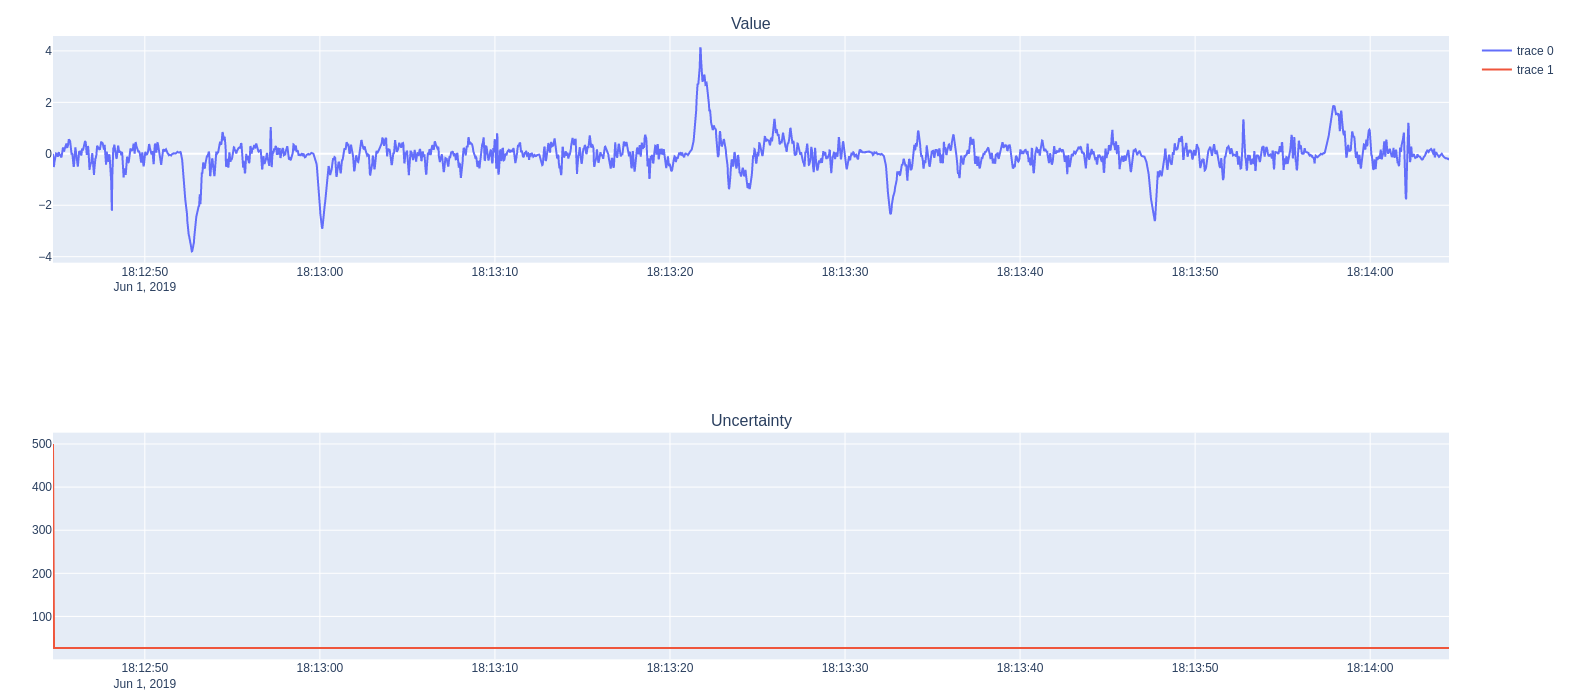
\includegraphics[width=\linewidth]{figures/vyw_uncertainty.png}\\
    \caption{Yaw rate state and uncertainty over time}
    \label{fig:vyw}
\end{figure}

\begin{figure}[H]
    \centering
    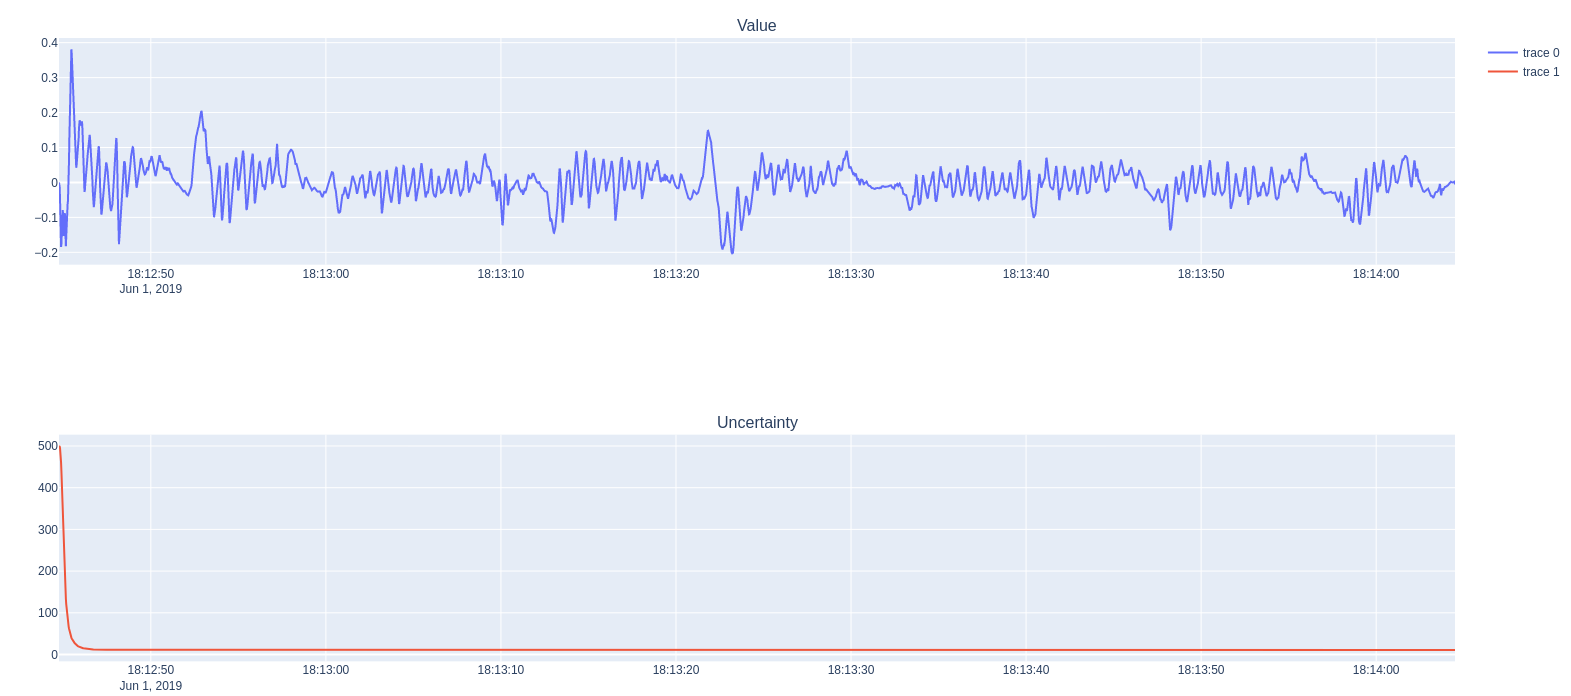
\includegraphics[width=\linewidth]{figures/rb_uncertainty.png}\\
    \caption{Roll bias state and uncertainty over time}
    \label{fig:rb}
\end{figure}
\begin{figure}[H]
    \centering
    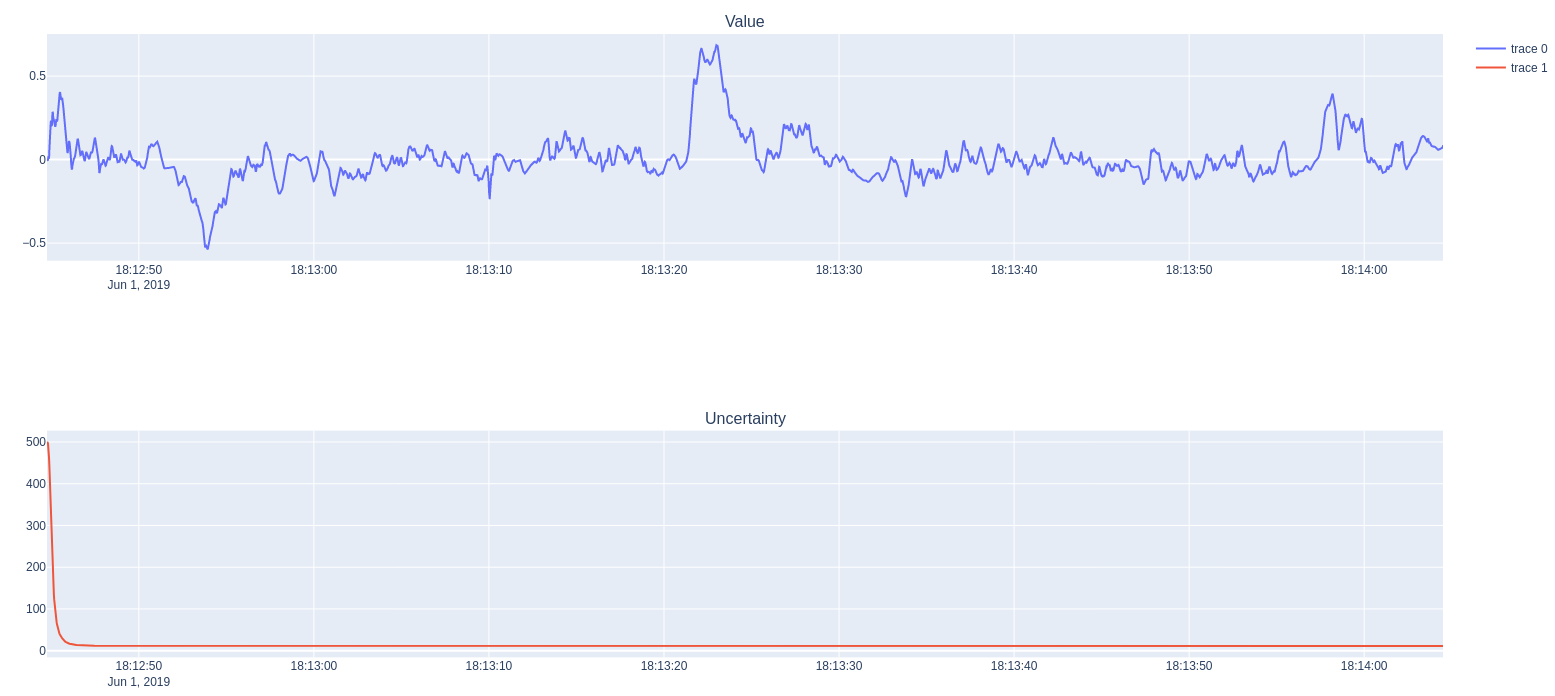
\includegraphics[width=\linewidth]{figures/pb_uncertainty.png}\\
    \caption{Pitch bias state and uncertainty over time}
    \label{fig:pb}
\end{figure}
\begin{figure}[H]
    \centering
    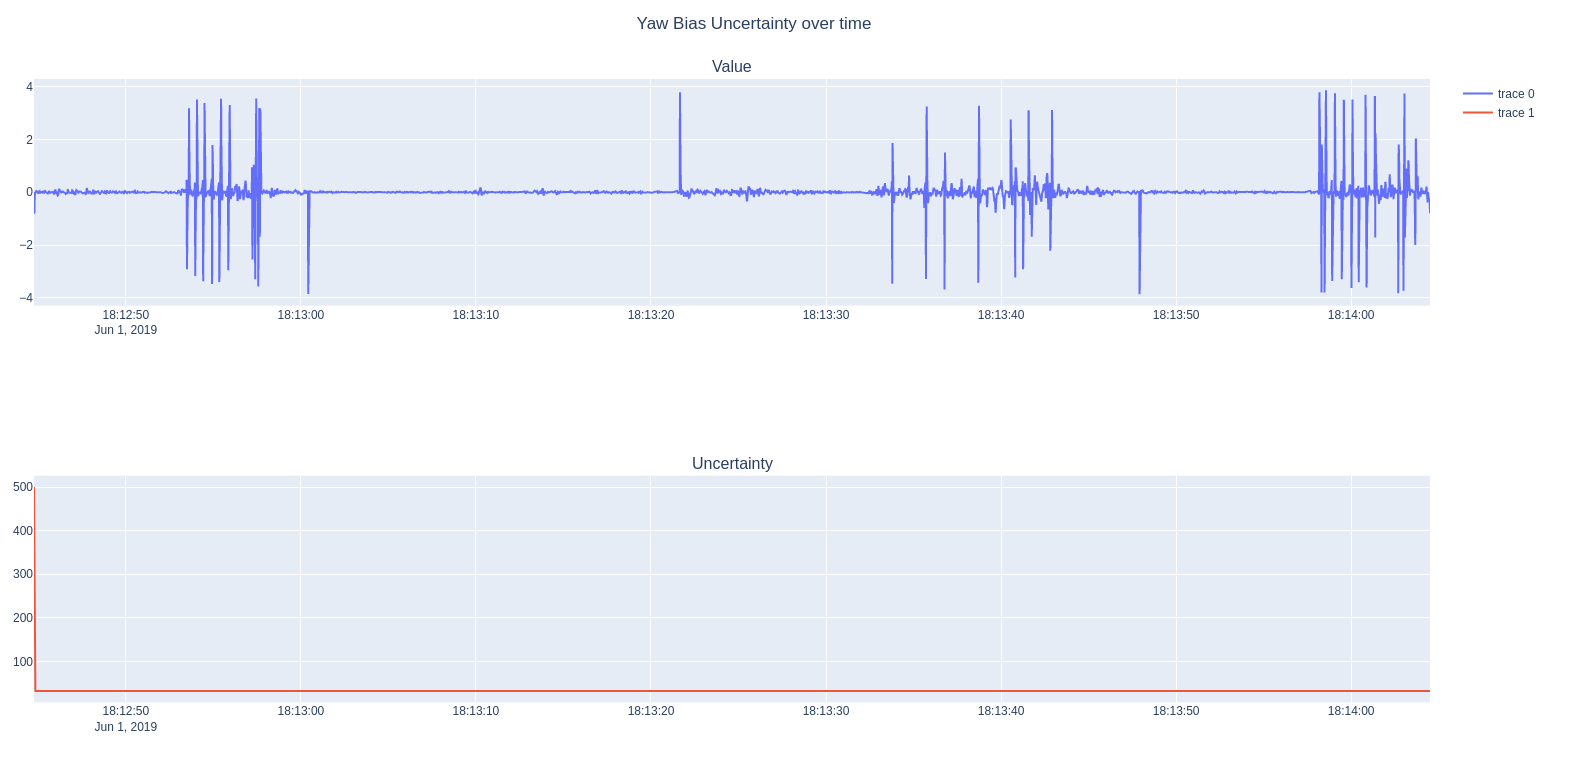
\includegraphics[width=\linewidth]{figures/yb_uncertainty.png}\\
    \caption{Yaw bias state and uncertainty over time}
    \label{fig:yb}
\end{figure}


\newpage
%=================================================================
%                           Appendix
%=================================================================
\section{Appendix}
\lhead{Appendix} % section header
\bibliography{citations.bib}
%=================================================================
%                           End Document
%=================================================================
\end{document}